

\subsection{Summary of the numerical results}

We conduct our experiments for $5$ different parameters  sets as presented in tables \ref{table:Reference solution, using MC with $500$ time steps, of Call option price under rBergomi model, for different parameter constellation.}. 

In Section \ref{sec:Weak error plots_no_change}, we estimate the weak error  (Bias) for the different parameter constellations, for $2$ scenarios involving with/without  Richardson extrapolation. The conclusions of this section are: 
\begin{itemize}
	\item Without Richardson extrapolation: For all cases except parameters set $4$, we get a weak error of order $\Delta t$, with different  constants. Interestingly, we see that the case of parameters set $4$ (see table \ref{table:Reference solution, using MC with $500$ time steps, of Call option price under rBergomi model, for different parameter constellation.}) has a weak error rate of order around $0.4$ but with a small constant. 
	
		\item With Richardson extrapolation: For all reported cases (sets  $1,2,3$ in table \ref{table:Reference solution, using MC with $500$ time steps, of Call option price under rBergomi model, for different parameter constellation.}), we get an improvement for weak error in terms of the rate and constants compared to the case without Richardson extrapolation.
\end{itemize}

\begin{remark}
We emphasize that the reported weak rates correspond to the pre-asymptotic regime that we are interested in. We are not interested on estimating the rates specifically but rather a sufficient precise estimate of the weak error (Bias), $\mathcal{E}_B(N)$, for different time steps $N$, in order to get the biased MC  solution for a given discretization, that we denoted $Q^N(\infty)$ in Section \ref{sec:Details of the MISC}.  For a fixed discretization, the corresponding biased solution will be set as a reference solution to the MISC solver in order to estimate the quadrature error $\mathcal{E}_Q(TOL_{\text{MISC}},N)$.	
\end{remark}

In Section \ref{sec:Comparing different  errors and complexity for MC and MISC}, we show tables and plots reporting  the different errors involved in MC method (bias and statistical error), related to the plots in Section \ref{sec:Weak error plots_no_change}, and in MISC (Quadrature error). We do this for each case of parameter set. The quadrature error (see \eqref{eq:quadrature error}) is computed by subtracting the MISC solution from the biased solution, computed with sufficiently large  number of samples (to kill the statistical error). Given that both methods, MC and MISC, have the same bias,  the computational time of MC and MISC is compared such that the statistical error is almost equal to the stable quadrature error produced by MISC.

 The conclusions of this section are: 


	\begin{enumerate}
		
		
		\item [i)] For the case of set $1$ (See Section \ref{sec:Case of set 1 parameters}), MISC coupled with Richardson extrapolation  is $3$ times faster than MC coupled with Richardson extrapolation, to achieve a total relative error around $8\%$  (see  tables(\ref{Total  error of MISC and MC to compute Call option price of the different tolerances for different number of time steps. Case set $1$ parameters, with Richardson extrapolation(level $1$). The numbers between parentheses are the corresponding absolute errors.}, \ref{Comparsion of the computational time of  MC and MISC, using Richardson extrapolation (level $1$), used to compute Call option price of rBergomi model for different number of time steps. Case set $1$ parameters})). This gain is improved when applying level $2$ Richardson extrapolation. In fact,  MISC coupled with Richardson extrapolation (level $2$) is $4$ times faster than MC coupled with Richardson extrapolation (level $2$), to achieve a total relative error around $0.5\%$ (see  tables  ( \ref{Total  error of MISC and MC to compute Call option price of the different tolerances for different number of time steps. Case set $1$ parameters, with Richardson extrapolation(level $2$). The numbers between parentheses are the corresponding absolute errors.}, \ref{Comparsion of the computational time of  MC and MISC, using Richardson extrapolation (level $2$), used to compute Call option price of rBergomi model for different number of time steps. Case set $1$ parameters})).  Applying Richardson extrapolation brought a significant improvement for MISC (compare tables (\ref{Total error of MISC and MC to compute Call option price of the different tolerances for different number of time steps. Case set 1, without Richardson extrapolation. The numbers between parentheses are the corresponding absolute errors.},\ref{Comparison of the computational time of  MC and MISC, used to compute Call option price of rBergomi model for different number of time steps. Case set1}) (no Richardson), tables (\ref{Total  error of MISC and MC to compute Call option price of the different tolerances for different number of time steps. Case set $1$ parameters, with Richardson extrapolation(level $1$). The numbers between parentheses are the corresponding absolute errors.}, \ref{Comparsion of the computational time of  MC and MISC, using Richardson extrapolation (level $1$), used to compute Call option price of rBergomi model for different number of time steps. Case set $1$ parameters}) (Richardson (level $1$)) and  tables ((\ref{Total  error of MISC and MC to compute Call option price of the different tolerances for different number of time steps. Case set $1$ parameters, with Richardson extrapolation(level $2$). The numbers between parentheses are the corresponding absolute errors.}, \ref{Comparsion of the computational time of  MC and MISC, using Richardson extrapolation (level $2$), used to compute Call option price of rBergomi model for different number of time steps. Case set $1$ parameters})) (Richardson (level $2$)), also see  figure \ref{fig:Complexity plot for  MISC for Case set $1$ parameters, comparison}).
		
			\item [ii)] For the case of set $2$ (See Section \ref{sec:Case of set $2$ parameters_linear}), MISC coupled with Richardson extrapolation is $19$ times faster than MC coupled with Richardson extrapolation, to achieve a total relative error around $8\%$ and $4$ times faster than MC, to achieve total relative error around $2\%$ (see tables (\ref{Total  error of MISC and MC to compute Call option price of the different tolerances for different number of time steps. Case set $2$ parameters, with Richardson extrapolation(level $1$). The numbers between parentheses are the corresponding absolute errors,relative},\ref{Comparsion of the computational time of  MC and MISC, using Richardson extrapolation (level $1$), used to compute Call option price of rBergomi model for different number of time steps. Case set $2$ parameters,linear})). This gain is improved when applying level $2$ Richardson extrapolation. In fact,  MISC coupled with Richardson extrapolation (level $2$) is $17$ times faster than MC coupled with Richardson extrapolation (level $2$), to achieve a total relative error below  $1\%$ (see  tables (\ref{Total  error of MISC and MC to compute Call option price of the different tolerances for different number of time steps. Case set $2$ parameters, with Richardson extrapolation(level $2$). The numbers between parentheses are the corresponding absolute errors,linear}, \ref{Comparsion of the computational time of  MC and MISC, using Richardson extrapolation (level $2$), used to compute Call option price of rBergomi model for different number of time steps. Case set $2$ parameters,linear})). Applying Richardson extrapolation brought a significant improvement for MISC (compare tables (\ref{Total error of MISC and MC to compute Call option price of the different tolerances for different number of time steps. Case $K=1$, $H=0.07$, without Richardson extrapolation. The numbers between parentheses are the corresponding absolute errors,linear}, \ref{Comparsion of the computational time of  MC and MISC, used to compute Call option price of rBergomi model for different number of time steps. Case $K=1, H=0.07$, linear}) (no Richardson), tables (\ref{Total  error of MISC and MC to compute Call option price of the different tolerances for different number of time steps. Case set $2$ parameters, with Richardson extrapolation(level $1$). The numbers between parentheses are the corresponding absolute errors,relative},\ref{Comparsion of the computational time of  MC and MISC, using Richardson extrapolation (level $1$), used to compute Call option price of rBergomi model for different number of time steps. Case set $2$ parameters,linear}) (Richardson (level $1$)) and  tables  (\ref{Total  error of MISC and MC to compute Call option price of the different tolerances for different number of time steps. Case set $2$ parameters, with Richardson extrapolation(level $2$). The numbers between parentheses are the corresponding absolute errors,linear}, \ref{Comparsion of the computational time of  MC and MISC, using Richardson extrapolation (level $2$), used to compute Call option price of rBergomi model for different number of time steps. Case set $2$ parameters,linear}) (Richardson (level $2$))).
		
		
		
		
			\item [iii)]  For the case of set $3$ (See Section \ref{sec:Case of set 3 parameters}), MISC is  $35$ times faster than MC, to achieve  a total relative error below $1\%$ and $8$ times faster than MC, to achieve a total relative error around $0.1\%$ (see figure \ref{fig:Complexity plot for MC and MISC for Case set $3$ parameters} and tables (\ref{Comparsion of the computational time of  MC and MISC, used to compute Call option price of rBergomi model for different number of time steps. Case set3}, \ref{Total error of MISC and MC to compute Call option price of the different tolerances for different number of time steps. Case set 3, without Richardson extrapolation. The numbers between parentheses are the corresponding absolute errors.})). Using Richardson extrapolation brought an improvement in terms of the  complexity constant compared to using simple MISC (See figure \ref{fig:Complexity plot for  MISC for case set $3$ parameters, comparison} and tables (\ref{Total  error of MISC and MC to compute Call option price of the different tolerances for different number of time steps. Case set $3$ parameters, with Richardson extrapolation(level $1$). The numbers between parentheses are the corresponding absolute errors.}, \ref{Comparsion of the computational time of  MC and MISC, using Richardson extrapolation (level $1$), used to compute Call option price of rBergomi model for different number of time steps. Case set $3$ parameters})).
				
	 	\item [iv)] For the case of set $4$ (See Section \ref{sec:Case of set 4 parameters}), MISC is  $141$ times faster than MC, to achieve a total relative error below $1\%$ (see figure \ref{fig:Complexity plot for MC and MISC for case set $4$ parameters} and tables (\ref{Comparsion of the computational time of  MC and MISC, used to compute Call option price of rBergomi model for different number of time steps. Case set4}, \ref{Total error of MISC and MC to compute Call option price of the different tolerances for different number of time steps. Case set 4, without Richardson extrapolation. The numbers between parentheses are the corresponding absolute errors.})).
		
	\item [v)] For the case of set $5$ (See Section \ref{sec:Case of set 5 parameters}), MISC is  $220$ times faster than MC, to achieve a total relative error below $6\%$ and $16$ times faster than MC, to achieve total relative error around $2\%$  (see figure \ref{fig:Complexity plot for MC and MISC for Case set $5$ parameters} and tables (\ref{Comparsion of the computational time of  MC and MISC, used to compute Call option price of rBergomi model for different number of time steps. Case set5}, \ref{Total error of MISC and MC to compute Call option price of the different tolerances for different number of time steps. Case set 5, without Richardson extrapolation. The numbers between parentheses are the corresponding absolute errors.})).
		
	\end{enumerate}

	
	











\subsection{Weak error plots} \label{sec:Weak error plots_no_change}
In this section, we include the results of weak errors for the different parameters sets as in table \ref{table:Reference solution, using MC with $500$ time steps, of Call option price under rBergomi model, for different parameter constellation.}, with and without Richardson extrapolation.  We considered a number of time steps $N \in \{2,4,8,16\}$.  The options are priced in terms of the moneyness $K$, where $K$ is the strike price.  The reference solution was computed with $N=500$ time steps (reported in table \ref{table:Reference solution, using MC with $500$ time steps, of Call option price under rBergomi model, for different parameter constellation.}). We note that the weak errors plotted here correspond to relative errors. We show in table \ref{table:Reference solution, using MC with $500$ time steps, of Call option price under rBergomi model, for different parameter constellation.} the different parameter constellations that we consider to report our results for MC and MISC.



\begin{table}[!h]
	\centering
	\begin{tabular}{l*{2}{c}r}
		Parameters            & Reference solution    \\
	Set $1$:	$H=0.43, K=1,S_0=1, \rho=-0.9, \eta=1.9,\xi=0.235^2$   & $\underset{(5.7e-05)}{0.0712074}$  \\	
			Set $2$:	$H=0.07, K=1,S_0=1, \rho=-0.9, \eta=1.9,\xi=0.235^2$   & $\underset{(7.9e-05)}{0.0790852}$  \\	

				Set $3$:	$H=0.02, K=1,,S_0=1, \rho=-0.7, \eta=0.4,\xi=0.1$   & $\underset{(1.3e-04)}{0.1247563}$  \\
					Set $4$:	$H=0.02, K=0.8,S_0=1, \rho=-0.7, \eta=0.4,\xi=0.1$   & $\underset{(5.6e-04)}{0.2407117}$  \\
						Set $5$:	$H=0.02, K=1.2,S_0=1, \rho=-0.7, \eta=0.4,\xi=0.1$   & $\underset{(2.5e-04)}{0.0568394}$  \\
		\hline
	\end{tabular}
	\caption{Reference solution, using MC with $500$ time steps and $M=10^6$, of call option price under rBergomi model, for different parameter constellation.  The numbers between parentheses correspond to the statistical errors.}
	\label{table:Reference solution, using MC with $500$ time steps, of Call option price under rBergomi model, for different parameter constellation.}
\end{table}
\FloatBarrier


\subsubsection{Without Richardson extrapolation}
From figures (\ref{fig:Weak_rate_set1_set_2_without_rich},\ref{fig:Weak_rate_H_002_without_rich_K_1_K_08},\ref{fig:Weak_rate_H_002_without_rich_K_12}), we see that for all cases  except parameters set $4$, we get a weak error of order $\Delta t$, with different  constants. Interestingly, we see that the case of parameters set $4$ (see table \ref{table:Reference solution, using MC with $500$ time steps, of Call option price under rBergomi model, for different parameter constellation.}) has a weak error rate of order around $0.4$ but with a small constant. The upper and lower bounds are $95\%$ confidence intervals.


\begin{figure}[h!]
	\centering
	\begin{subfigure}{.4\textwidth}
		\centering
		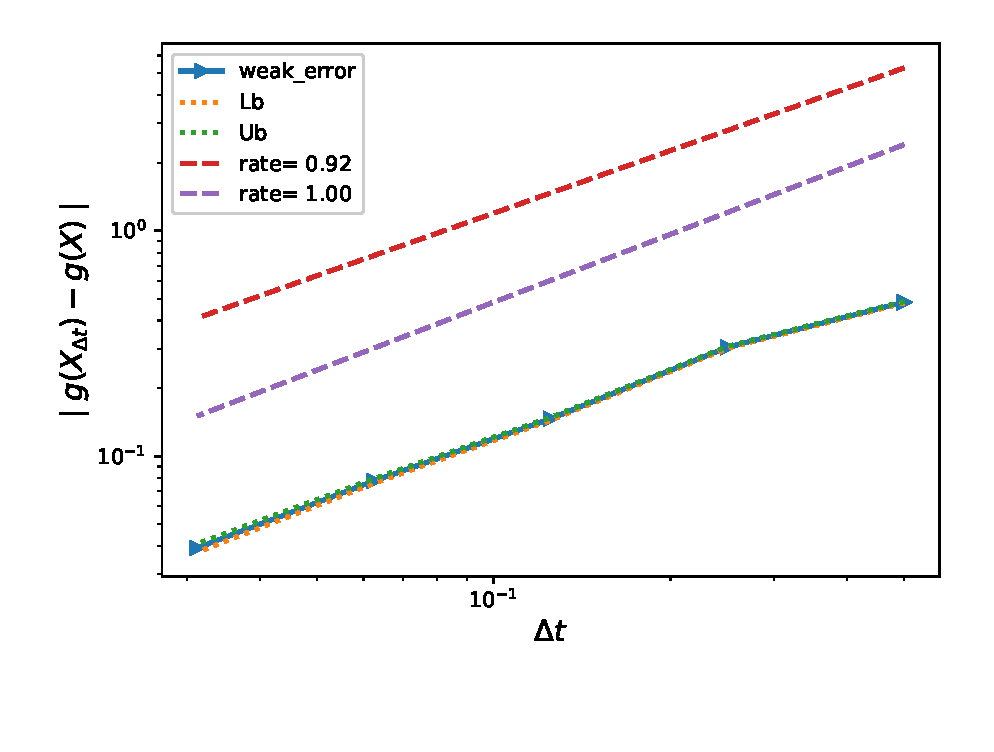
\includegraphics[width=1\linewidth]{./figures/rBergomi_weak_error_rates/without_richardson/H_043/weak_convergence_order_Bergomi_H_043_K_1_M_10_6_CI_relative}
		\caption{}
		\label{fig:sub3}
	\end{subfigure}%
	\begin{subfigure}{.4\textwidth}
		\centering
		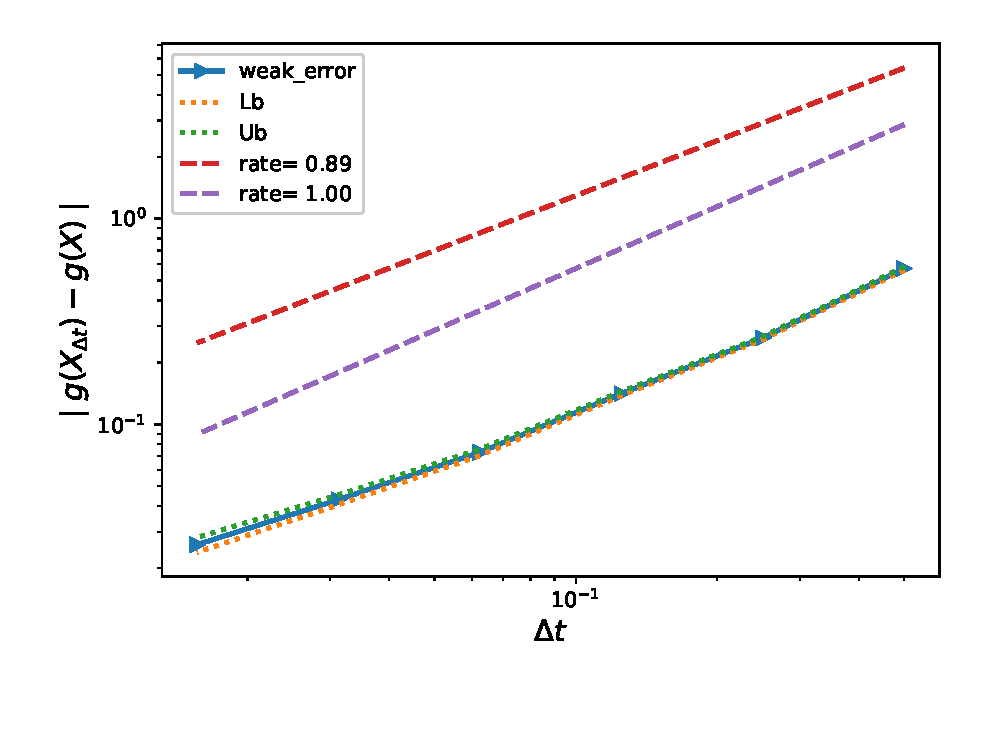
\includegraphics[width=1\linewidth]{./figures/rBergomi_weak_error_rates/without_richardson/H_007/weak_convergence_order_Bergomi_H_007_K_1_M_10_6_CI_relative}
		\caption{}
		\label{fig:sub4}
	\end{subfigure}
	
	\caption{The rate of convergence of the weak error  $\abs{\expt{g(X_{\Delta t})}-g(X)}$  without Richardson extraploation, using MC with $M=10^6$: a) Set $1$ parameters in table \ref{table:Reference solution, using MC with $500$ time steps, of Call option price under rBergomi model, for different parameter constellation.}.  b) Set $2$ parameters in table \ref{table:Reference solution, using MC with $500$ time steps, of Call option price under rBergomi model, for different parameter constellation.}.}
	\label{fig:Weak_rate_set1_set_2_without_rich}
\end{figure}





\begin{figure}[!htb]
	\centering
	\begin{subfigure}{.4\textwidth}
		\centering
		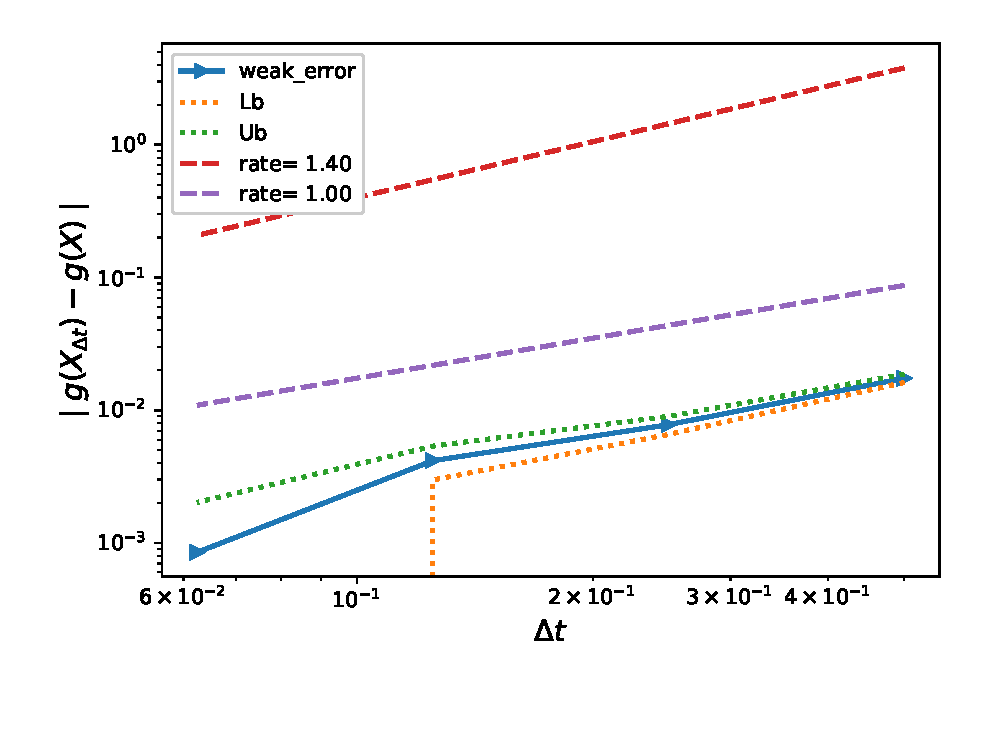
\includegraphics[width=1\linewidth]{./figures/rBergomi_weak_error_rates/without_richardson/H_002/weak_convergence_order_Bergomi_H_002_K_1_M_3_10_6_CI_relative}
		\caption{}
		\label{fig:sub3}
	\end{subfigure}%
	\begin{subfigure}{.4\textwidth}
		\centering
		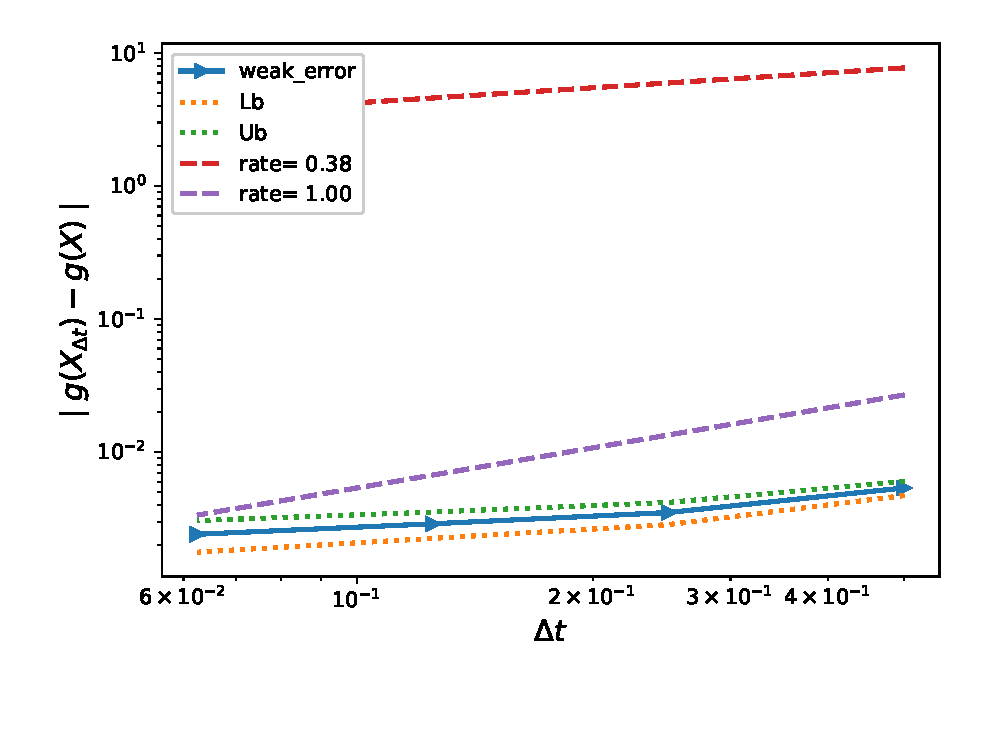
\includegraphics[width=1\linewidth]{./figures/rBergomi_weak_error_rates/without_richardson/H_002/weak_convergence_order_Bergomi_H_002_K_08_M_5_10_6_CI_relative}
		\caption{}
		\label{fig:sub4}
	\end{subfigure}
	
	\caption{The rate of convergence of the weak error $\abs{\expt{g(X_{\Delta t})}-g(X)}$  without Richardson extraploation, using MC with $M=5.10^6$: a) Set $3$ parameters in table \ref{table:Reference solution, using MC with $500$ time steps, of Call option price under rBergomi model, for different parameter constellation.},  b) Set $4$ parameters in table \ref{table:Reference solution, using MC with $500$ time steps, of Call option price under rBergomi model, for different parameter constellation.}. }
	\label{fig:Weak_rate_H_002_without_rich_K_1_K_08}
\end{figure}











\begin{figure}[!htb]
		\centering
		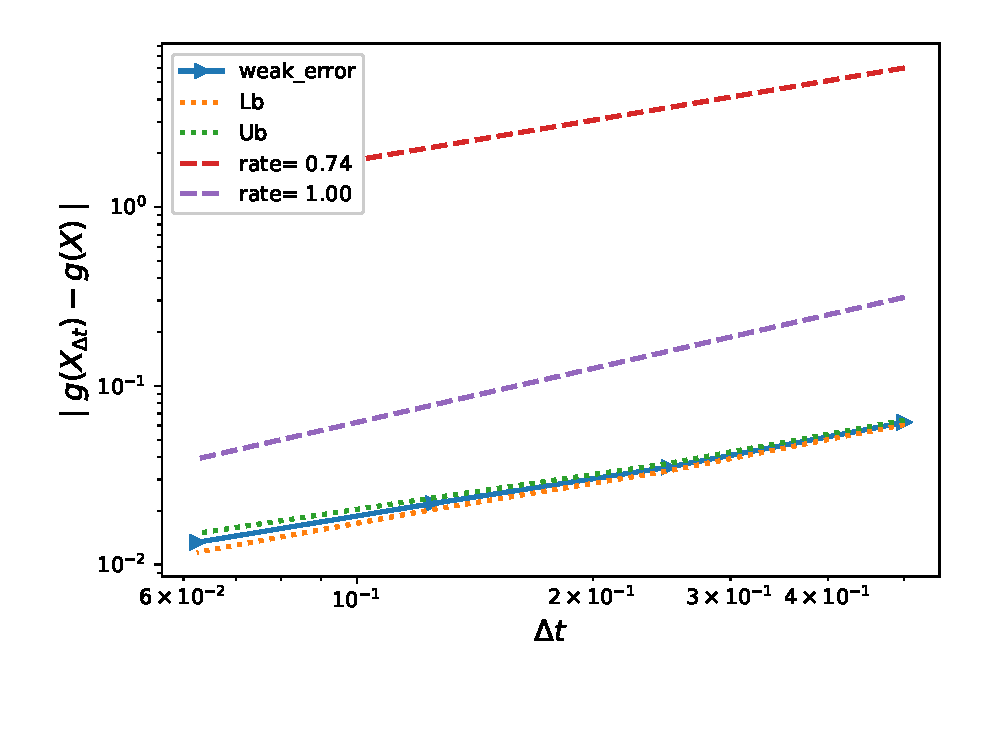
\includegraphics[width=0.4\linewidth]{./figures/rBergomi_weak_error_rates/without_richardson/H_002/weak_convergence_order_Bergomi_H_002_K_12_M_3_10_6_CI_relative}	
	\caption{The rate of convergence of the weak error $\abs{\expt{g(X_{\Delta t})}-g(X)}$, for set $5$ parameters in table \ref{table:Reference solution, using MC with $500$ time steps, of Call option price under rBergomi model, for different parameter constellation.}, without Richardson extraploation, using MC with $M=5.10^6$.}
	\label{fig:Weak_rate_H_002_without_rich_K_12}
\end{figure}


\FloatBarrier


\subsubsection{With Richardson extrapolation (level 1)}
Figures (\ref{fig:Weak_rate_H_043_007_with_rich}, \ref{fig:Weak_rate_H_002_with_rich_K1}) illustrate the weak errors estimates for parameters sets $1,2,3$ in table \ref{table:Reference solution, using MC with $500$ time steps, of Call option price under rBergomi model, for different parameter constellation.}. The upper and lower bounds are $95\%$ confidence intervals.
\begin{figure}[h!]
	\centering
	\begin{subfigure}{.4\textwidth}
		\centering
		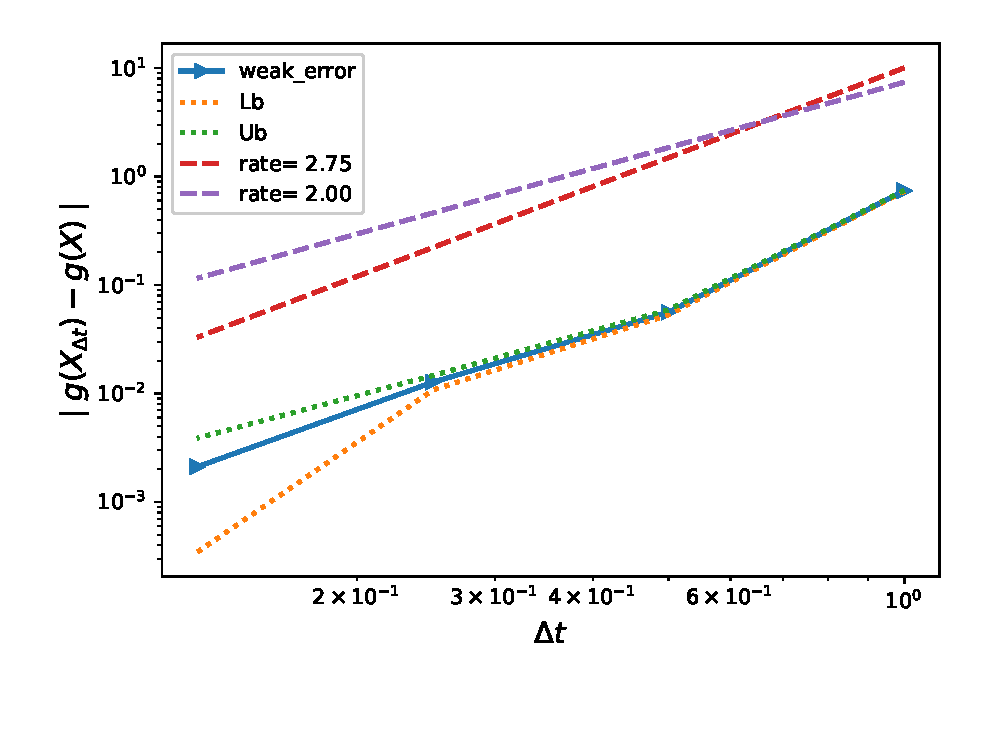
\includegraphics[width=1\linewidth]{./figures/rBergomi_weak_error_rates/with_richardson/H_043/weak_convergence_order_Bergomi_H_043_K_1_M_10_6_richardson_relative}
		\caption{}
		\label{fig:sub3}
	\end{subfigure}%
	\begin{subfigure}{.4\textwidth}
		\centering
		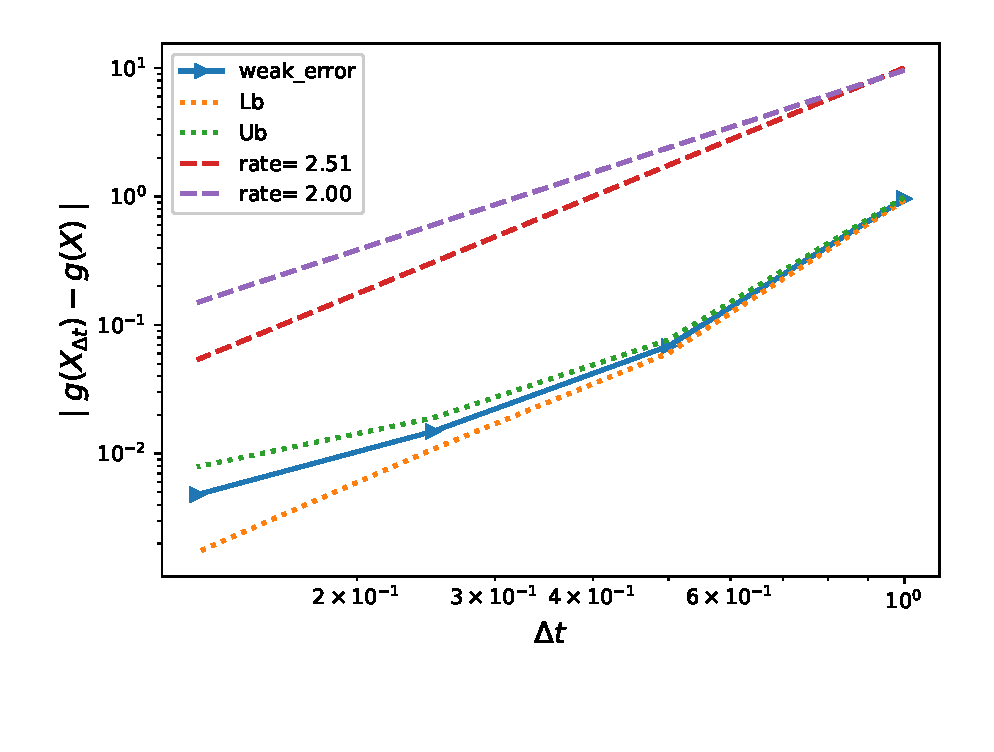
\includegraphics[width=1\linewidth]{./figures/rBergomi_weak_error_rates/with_richardson/H_007/weak_convergence_order_Bergomi_H_007_K_1_richardson_relative_M_10_6}
		\caption{}
		\label{fig:sub4}
	\end{subfigure}
	
	\caption{The rate of convergence of the weak error  $\abs{\expt{2 g(X_{\Delta t/2}) -g(X_{\Delta t})}-g(X)}$   with Richardson extraploation, using MC with $M=10^6$: a) Set $1$ parameters in table \ref{table:Reference solution, using MC with $500$ time steps, of Call option price under rBergomi model, for different parameter constellation.}.  b) Set $2$ parameters in table \ref{table:Reference solution, using MC with $500$ time steps, of Call option price under rBergomi model, for different parameter constellation.}, }
	\label{fig:Weak_rate_H_043_007_with_rich}
\end{figure}




\begin{figure}[!htbp]
	\centering
		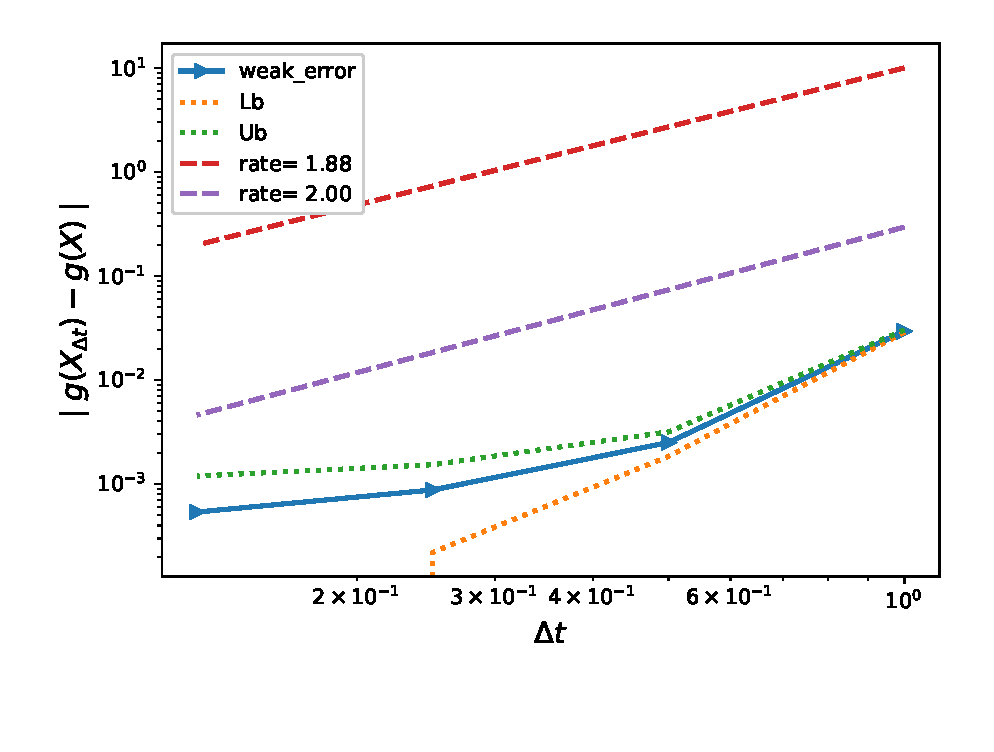
\includegraphics[width=0.4\linewidth]{./figures/rBergomi_weak_error_rates/with_richardson/H_002/weak_convergence_order_Bergomi_H_002_K_1_M_1_10_7_richardson_relative}
	\caption{The rate of convergence of the weak error $\abs{\expt{2 g(X_{\Delta t/2}) -g(X_{\Delta t})}-g(X)}$,  for set $3$ parameters in table \ref{table:Reference solution, using MC with $500$ time steps, of Call option price under rBergomi model, for different parameter constellation.}, with Richardson extraploation, using MC with $M=10^7$. }
	\label{fig:Weak_rate_H_002_with_rich_K1}
\end{figure}
\FloatBarrier




\subsection{Comparing different  errors and complexity for MC and MISC}\label{sec:Comparing different  errors and complexity for MC and MISC}


The results were reported for the different sets of parameters defined in table \ref{table:Reference solution, using MC with $500$ time steps, of Call option price under rBergomi model, for different parameter constellation.}. We considered   a number of time steps $N \in \{2,4,8,16\}$.  The options are priced in terms of the moneyness $K$, where $K$ is the strike price.   

 For each set,  we report the results for $2$ scenarios: i) Without using Richardson extrapolation and  ii) Using level $1$ Richardson extrapoaltion.

In each case, we show a table of computed values using MISC with different tolerances as well the biased MC value, using large number of samples to kill the statistical error. Then, in a second table,  we show the bias as well the statistical error for MC method, related to Section \ref{sec:Weak error plots_no_change}. After that, a plot  shows the behavior of  the relative quadrature error which is computed as the normalized difference between the biased MC solution and MISC solution. Then, we provide the total relative error which is the sum of the bias and statistical error for MC, and the quadrature error for MISC. We note that we used a number of samples for MC such that the statistical error is almost equal to the stable quadrature error, in order to have a fair complexity comparison between the two methods. Finally, we show the CPU time needed for each solver. We note that  in all cases the actual work (runtime) was obtained using a $40$-core Intel(R) Xeon(R) CPU E5-268 architecture.

\subsubsection{Case of set $1$ parameters in table \ref{table:Reference solution, using MC with $500$ time steps, of Call option price under rBergomi model, for different parameter constellation.}}\label{sec:Case of set 1 parameters}

\subsubsection*{Without Richardson extrapolation}
\begin{table}[h!]
	\centering
	\begin{tabular}{l*{6}{c}r}
		Method \textbackslash  Steps            & $2$ & $4$ & $8$ & $16$ &   \\
		\hline
%		MISC ($TOL_{\text{MISC}}=5.10^{-1}$)  & $0.1140$ & $0.0961$ & $0.0848$ & $0.0781$  \\
		MISC ($TOL_{\text{MISC}}=10^{-1}$)  & $0.1140$ & $0.0961$ & $0.0871$ & $0.0802$  \\
%		MISC ($TOL_{\text{MISC}}=5.10^{-2}$)  & $0.1140$ & $0.0963$ & $0.0843$ & $0.0824$  \\
		MISC ($TOL_{\text{MISC}}=10^{-2}$)  & $0.1077$ & $0.0944$ & $0.0838$ & $0.0772$  \\

		MISC ($TOL_{\text{MISC}}=10^{-3}$)  & $0.1077$ & $0.0921$ & $0.0819$ & $0.0762$  \\
%		MISC ($TOL_{\text{MISC}}=5.10^{-4}$)  & $0.1079   $ & $0.0921$ & $0.0822$ & $0.0762$  \\
		MISC ($TOL_{\text{MISC}}=10^{-4}$)  & $0.1079$ & $0.0921$ & $0.0822$ & $-$  \\
		\hline
		MC method ($M=8.10^{6}$)   & $  0.1078$ & $ 0.0921
		$  & $   0.0822
		$ & $ 0.0767$ \\		
		
		\hline
	\end{tabular}
	\caption{ Call option price of the different methods for different number of time steps. Case of set $1$ parameters in table \ref{table:Reference solution, using MC with $500$ time steps, of Call option price under rBergomi model, for different parameter constellation.}, without Richardson extrapolation.}
	\label{table: Call option price of the different methods for different number of time steps. Case set 1}
\end{table}


\begin{table}[h!]
	\centering
	\begin{tabular}{l*{6}{c}r}
		Method \textbackslash  Steps            & $2$ & $4$ & $8$ & $16$  \\
		\hline
		MC Bias ($M=8.10^6$)   & 	$ \underset{( 0.0366)}{\mathbf{0.5142}}$  & $\underset{( 0.0209)}{\mathbf{0.2933}}$  & $\underset{( 0.0110)}{\mathbf{0.1551}}$ & $\underset{( 0.0055)}{\mathbf{0.0777}}$\\ 
		
		MC Statistical error ($M=8.10^6$)  &  $\underset{(  6.0e-05)} {\mathbf{8.4e-04}}$  & $\underset{(3.4e-05)} {\mathbf{4.8e-04}}$  & $\underset{(2.7e-05)} {\mathbf{ 3.8e-04}}$ & $\underset{( 2.35e-05)} {\mathbf{3.3e-04}}$	\\

		\hline
	\end{tabular}
	\caption{Bias and statistical errors of MC  for computing call option price  for different number of time steps. Case set $1$, without Richardson extrapolation. The numbers between parentheses are the corresponding absolute errors.}
	\label{Bias and Statistical errors of MC ($M=10^6$)  for computing Call option price  for different number of time steps. Case set 1, without Richardson extrapolation. The numbers between parentheses are the corresponding absolute errors.}
\end{table}








\begin{figure}[h!]
	\centering
	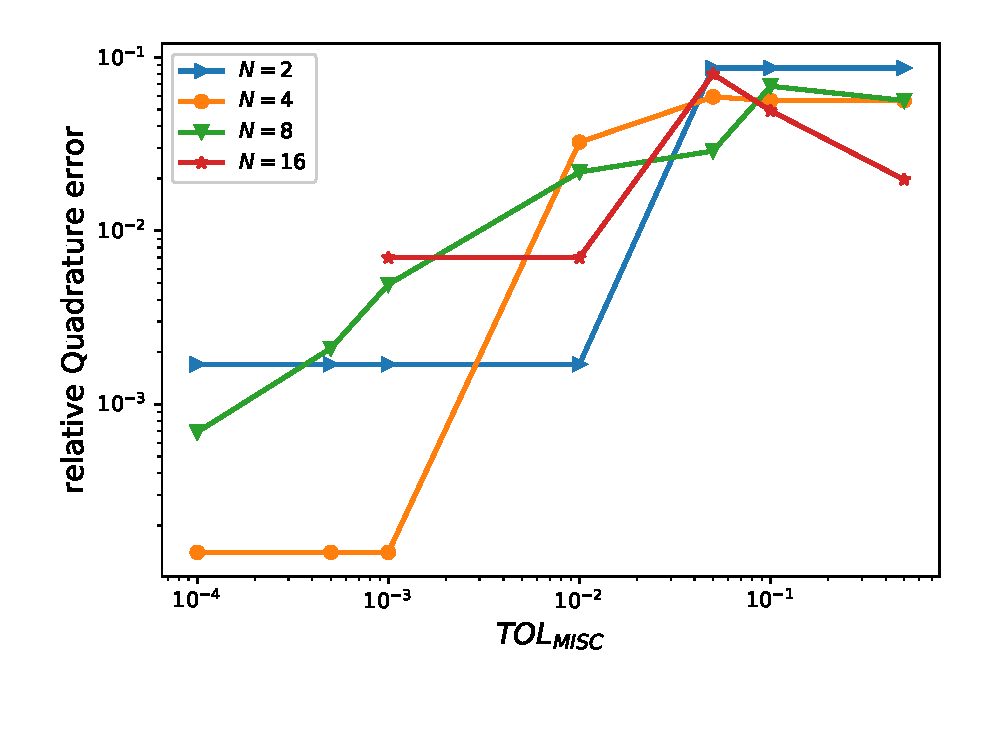
\includegraphics[width=0.5\linewidth]{./figures/rBergomi_MISC_quadratre_error/vs_TOL/set1/relative_quad_error_wrt_MISC_TOL_set1_non_rich}
	
	
	\caption{Quadrature error of MISC, with different tolerances, to compute call option price for different number of time steps. Case  set $1$ parameters, without Richardson extrapolation. See detailed values  in table \ref{Quadrature error of MISC to compute Call option price of the different tolerances for different number of time steps. Case  set $1$ parameters, without Richardson extrapolation. The numbers between parentheses are the corresponding absolute errors.}}
	\label{fig:Quadrature_error_set1}
\end{figure}




\begin{table}[h!]
	\centering
	\begin{tabular}{l*{6}{c}r}
		Method \textbackslash  Steps            & $2$ & $4$ & $8$ & $16$  \\
		\hline
%		MISC ($TOL_{\text{MISC}}=5.10^{-1}$)  & $\mathbf{0.6010}$ & $\mathbf{0.3496}$ & $\mathbf{ 0.2114}$ & $\mathbf{ 0.0974}$  \\
		MISC ($TOL_{\text{MISC}}=10^{-1}$)  & $\mathbf{0.6010}$ & $\mathbf{0.3496}$ & $\mathbf{  0.2232}$ & $\mathbf{
			0.1269}$  \\
%		MISC ($TOL_{\text{MISC}}=5.10^{-2}$)  &$\mathbf{0.6010}$ & $\mathbf{  0.3524}$ & $\mathbf{ 0.1839}$ & $\mathbf{  0.1577}$  \\
		MISC ($TOL_{\text{MISC}}=10^{-2}$)  & $\mathbf{\red{0.5159}}$ & $\mathbf{0.3257}$ & $\mathbf{ 0.1769}$ & $\mathbf{  \red{0.0847}}$  \\
		MISC ($TOL_{\text{MISC}}=10^{-3}$)  & $\mathbf{0.5159}$ & $\mathbf{\red{0.2934}}$ & $\mathbf{0.1600}$ & $\mathbf{0.0847}$  \\
%		MISC ($TOL_{\text{MISC}}=5.10^{-4}$)  & $\mathbf{0.5159}$ & $\mathbf{0.2934}$ & $\mathbf{0.1572}$ & $\mathbf{-}$  \\
		MISC ($TOL_{\text{MISC}}=10^{-4}$)  & $\mathbf{0.5159}$ & $\mathbf{0.2934}$ & $\mathbf{\red{0.1558}}$ & $\mathbf{-}$  \\
		\hline
		MC     & $\mathbf{\red{0.5159}}$ & $\mathbf{\red{0.2938}}$ & $\mathbf{\red{0.1555}}$ &$\mathbf{  \red{0.0817}}$  \\	
		
		\hline
	\end{tabular}
	\caption{Total relative error of MISC, with different tolerances,  and MC to compute call option price for different number of time steps. Case  set $1$ parametrs of table \ref{table:Reference solution, using MC with $500$ time steps, of Call option price under rBergomi model, for different parameter constellation.}, without Richardson extrapolation. The values marked in red, for MISC method, correspond to the total relative errors associated with  stable quadrature errors for MISC, and will be used for complexity comparison against MC.}
	\label{Total error of MISC and MC to compute Call option price of the different tolerances for different number of time steps. Case set 1, without Richardson extrapolation. The numbers between parentheses are the corresponding absolute errors.}
\end{table}



\begin{table}[h!]
	\centering
	\begin{tabular}{l*{6}{c}r}
		Method \textbackslash  Steps            & $2$ & $4$ & $8$ & $16$ &   \\
		\hline
%		MISC ($TOL_{\text{MISC}}=5.10^{-1}$)  & $0.1$ & $0.1$ & $0.2$ & $0.4$  \\
		MISC ($TOL_{\text{MISC}}=10^{-1}$)  & $0.1$ & $0.1$ & $0.6$ & $6$  \\
%		MISC ($TOL_{\text{MISC}}=5.10^{-2}$)  & $0.1$ & $0.3$ & $2$ & $14$  \\
		MISC ($TOL_{\text{MISC}}=10^{-2}$)  & $\red{0.2}$ & $1$ & $9$ & $\red{215}$  \\
		MISC ($TOL_{\text{MISC}}=10^{-3}$)  & $2$ & $\red{11}$ & $243$ & $4650$  \\
%		MISC ($TOL_{\text{MISC}}=5.10^{-4}$)  & $3$ & $17$ & $ 670$ & $-$  \\
		MISC ($TOL_{\text{MISC}}=10^{-4}$)  & $6$ & $96$ & $\red{5760}$ & $-$  \\
		\hline
		MC     & $\red{ 50}$  & $\red{344}$  & $\red{637}$ & $\red{8}$  \\
		
		\hline
		Ratio of $\left(\text{MC}/ \text{MISC} \right)$  &$\red{  250}$ & $\red{    31
		}$  & $\red{ 0.1
		}$  & $\red{  0.04}$ \\
		\hline
	\end{tabular}
	\caption{Comparison of the computational time (in Seconds) of  MC and MISC, used to compute call option price of rBergomi model for different number of time steps. Case set $1$ parametrs of table \ref{table:Reference solution, using MC with $500$ time steps, of Call option price under rBergomi model, for different parameter constellation.}. The
		average MC CPU time is computed over 10 runs. }
	\label{Comparison of the computational time of  MC and MISC, used to compute Call option price of rBergomi model for different number of time steps. Case set1}
\end{table}

\subsubsection*{With Richardson extrapolation (level $1$)}







\begin{table}[h!]
	\centering
	\begin{tabular}{l*{6}{c}r}
		Method \textbackslash  Steps    &$1-2$         & $2-4$ & $4-8$ \\
		\hline
%		MISC ($TOL_{\text{MISC}}=5.10^{-1}$)& $0.1357$  & $0.0783$ & $0.0735$ \\
		MISC ($TOL_{\text{MISC}}=10^{-1}$)  &$0.1357$  &$0.0783$ & $0.0785$   \\
%		MISC ($TOL_{\text{MISC}}=5.10^{-2}$)  & $0.1357$ & $0.0831$ & $0.0773$   \\
		MISC ($TOL_{\text{MISC}}=10^{-2}$)  & $0.1237$ &$0.0781$ & $0.0745$   \\

		MISC ($TOL_{\text{MISC}}=10^{-3}$)  & $0.1224$ &$0.0766$ & $0.0720$  \\
		MISC ($TOL_{\text{MISC}}=10^{-4}$)  &$0.1224$ & $0.0763$ & $0.0724$ \\
		\hline
		MC method ($M=10^6$)  &$	0.1237$ & $0.0752$ & $0.0721$ \\
		\hline
	\end{tabular}
	\caption{Call option price of the different methods for different number of time steps. Case set $1$ parameters of table \ref{table:Reference solution, using MC with $500$ time steps, of Call option price under rBergomi model, for different parameter constellation.}, using Richardson extrapolation (level $1$).}
	\label{table:  Call option price of the different methods for different number of time steps. Case set $1$ parameter, using Richardson extrapolation (level $1$)}
\end{table}




\begin{table}[h!]
	\centering
	\begin{tabular}{l*{6}{c}r}
		Method \textbackslash  Steps            & $1-2$ & $2-4$ & $4-8$ & $8-16$  \\
		\hline
		MC  Bias ($M=10^6$)    &$\underset{( 0.0525)}{\mathbf{0.7378}}$  & $\underset{(    0.0040)}{\mathbf{0.0561}}$  & $\underset{(0.0009 )}{\mathbf{0.0127}}$  & $\underset{(0.0001)}{\mathbf{0.0021}}$ \\	
		
		MC Statistical error ($M=10^6$)   & $\underset{( 2.3e-04)}{\mathbf{3.3e-03}}$  & $\underset{(  1.1e-04)}{\mathbf{1.6e-03}}$  & $\underset{(7.1e-05)}{\mathbf{1.0e-03}}$ & $\underset{(   6.4e-05 )}{\mathbf{9.0e-04}}$ \\	
		
		
		\hline
	\end{tabular}
	\caption{Bias and statistical errors of MC   for computing call option price  for different number of time steps. Case set $1$ parameters in tabel \ref{table:Reference solution, using MC with $500$ time steps, of Call option price under rBergomi model, for different parameter constellation.}, with Richardson extrapolation (level $1$). The numbers between parentheses are the corresponding absolute errors.}
	\label{Bias and Statistical errors of MC ($M=10^6$)  for computing Call option price  for different number of time steps. Case set $1$ parameters, with Richardson extrapolation (level1). The numbers between parentheses are the corresponding absolute errors.}
\end{table}








\begin{figure}[h!]
	\centering
	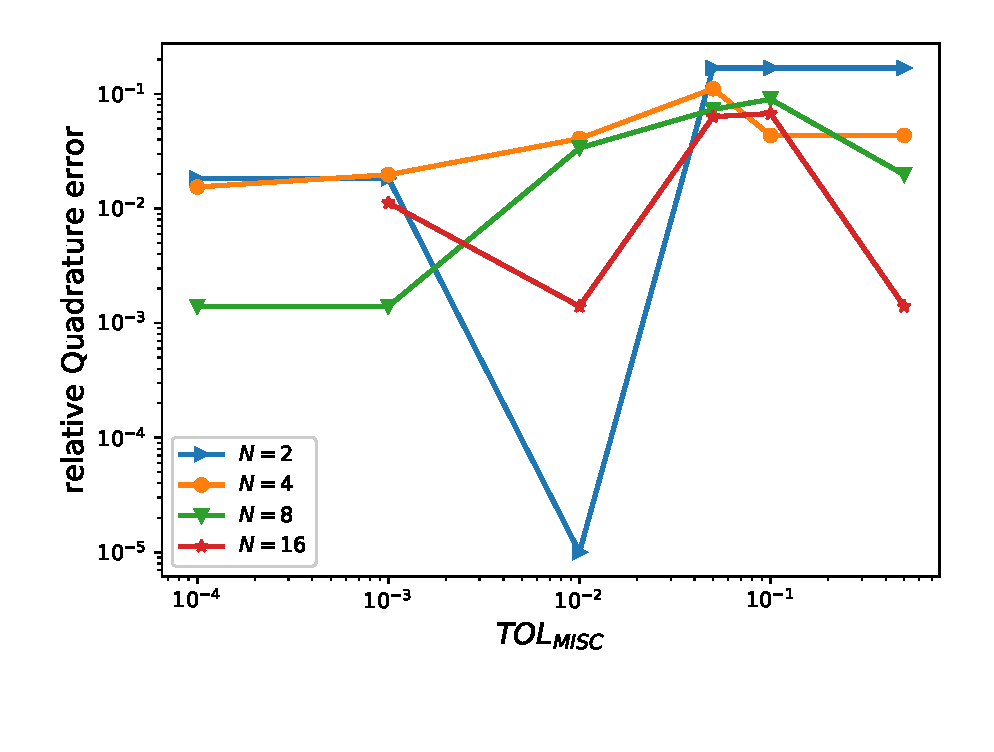
\includegraphics[width=0.5\linewidth]{./figures/rBergomi_MISC_quadratre_error/vs_TOL/set1/relative_quad_error_wrt_MISC_TOL_set1_with_rich}
	
	
	\caption{Quadrature error of MISC, with different tolerances, to compute call option price for different number of time steps. Case  set $1$ parameters, with Richardson extrapolation.  See detailed values  in table \ref{Quadrature error of MISC to compute Call option price of the different tolerances for different number of time steps. Case set $1$ parameters, with Richardson extrapolation(level $1$). The numbers between parentheses are the corresponding absolute errors.}.}
\end{figure}



\begin{table}[!h]
	\centering
	\begin{tabular}{l*{6}{c}r}
		Method \textbackslash  Steps            & $1-2$ & $2-4$ & $4-8$   \\
		\hline
%		MISC ($TOL_{\text{MISC}}=5.10^{-1}$)  & $\mathbf{0.9063
%		}$ & $\mathbf{ 0.0996}$ & $\mathbf{0.0324
%		}$  \\
		MISC ($TOL_{\text{MISC}}=10^{-1}$)  & $\mathbf{0.9063
		}$ & $\mathbf{ 0.0996}$ & $\mathbf{  0.1026}$   \\
%		MISC ($TOL_{\text{MISC}}=5.10^{-2}$)  & $\mathbf{0.9063
%		}$ & $\mathbf{    0.1670}$ & $\mathbf{ 0.0857}$  \\
		MISC ($TOL_{\text{MISC}}=10^{-2}$)  & $\mathbf{0.7378}$ & $\mathbf{  0.0968}$ & $\mathbf{   0.0464}$  \\	
		MISC ($TOL_{\text{MISC}}=10^{-3}$)  & $\mathbf{\red{0.7561}}$ & $\mathbf{\red{0.0758}}$ & $\mathbf{\red{0.0141}}$  \\
		MISC ($TOL_{\text{MISC}}=10^{-4}$)  & $\mathbf{0.7561}$ & $\mathbf{0.0715}$ & $\mathbf{0.0141}$ \\
		\hline
		MC   & $\mathbf{\red{0.7561}}$  & $\mathbf{\red{0.0758}}$  & $\mathbf{\red{0.0141}}$  \\
		
		\hline
	\end{tabular}
	\caption{Total  relative error of MISC and MC, with different tolerances, to compute call option price for different number of time steps. Case set $1$ parameters in table \ref{table:Reference solution, using MC with $500$ time steps, of Call option price under rBergomi model, for different parameter constellation.}, with Richardson extrapolation(level $1$). The values marked in red, for MISC method, correspond to the total relative errors associated with  stable quadrature errors for MISC, and will be used for complexity comparison against MC.}
	\label{Total  error of MISC and MC to compute Call option price of the different tolerances for different number of time steps. Case set $1$ parameters, with Richardson extrapolation(level $1$). The numbers between parentheses are the corresponding absolute errors.}
\end{table}

\begin{table}[!h]
	\centering
	\begin{tabular}{l*{6}{c}r}
		Method \textbackslash  Steps            & $1-2$ & $2-4$ & $4-8$   \\
		\hline
%		MISC ($TOL_{\text{MISC}}=5.10^{-1}$)  & $0.1$ & $0.1$ & $0.2$  \\
		MISC ($TOL_{\text{MISC}}=10^{-1}$)  & $0.1$ & $0.1$ & $0.6$ \\
%		MISC ($TOL_{\text{MISC}}=5.10^{-2}$)  & $0.1$ & $0.4$ & $2$   \\
		MISC ($TOL_{\text{MISC}}=10^{-2}$)  & $1$ & $2$ & $18$   \\
		MISC ($TOL_{\text{MISC}}=10^{-3}$)  & $\red{4}$ & $\red{12}$ & $\red{520}$   \\	
		MISC ($TOL_{\text{MISC}}=10^{-4}$)  & $7$ & $191$ & $7650$  \\
		\hline
		MC   & $\red{ 34.7}$  & $\red{37}$  & $ \red{532}$    \\
		
		\hline
		Ratio of $\left(\text{MC}/ \text{MISC} \right)$  &$\red{8.7}$ & $\red{   3.1
		}$  & $\red{1}$ \\
		\hline
	\end{tabular}
	\caption{Comparison of the computational time (in Seconds) of  MC and MISC, using Richardson extrapolation (level $1$), used to compute call option price of rBergomi model for different number of time steps. Case set $1$ parameters in table \ref{table:Reference solution, using MC with $500$ time steps, of Call option price under rBergomi model, for different parameter constellation.}. The
		average MC CPU time is computed over 10 runs.}
	\label{Comparsion of the computational time of  MC and MISC, using Richardson extrapolation (level $1$), used to compute Call option price of rBergomi model for different number of time steps. Case set $1$ parameters}
\end{table}



\begin{figure}[h!]
	\centering
	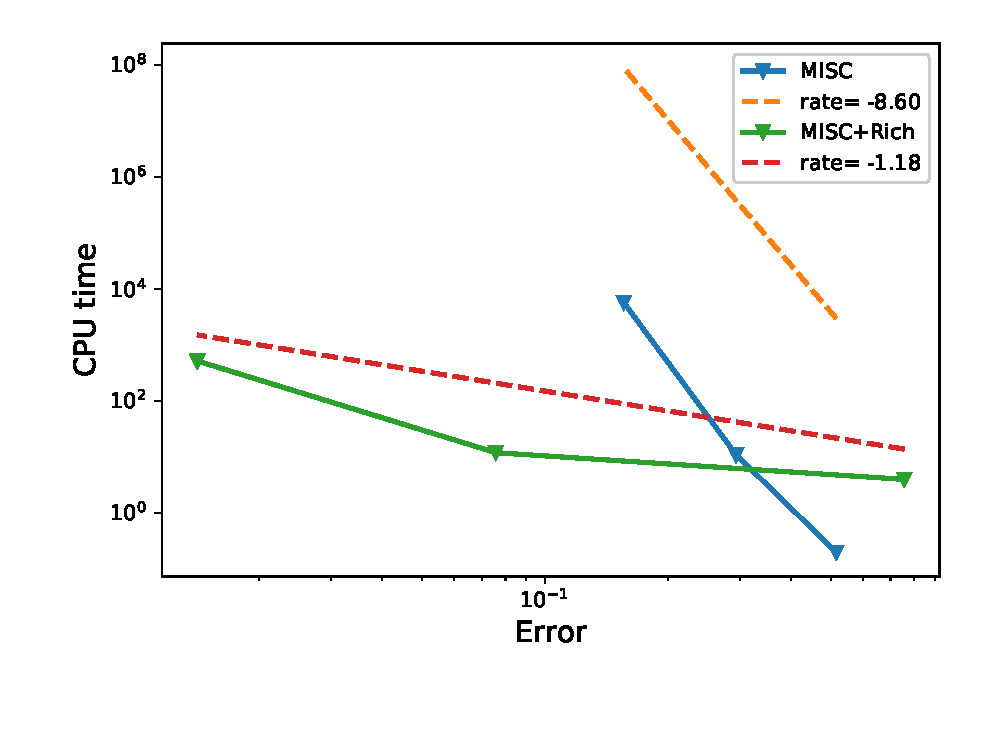
\includegraphics[width=0.5\linewidth]{./figures/rBergomi_Complexity_rates/set1/error_vs_time_set1_comparison}
	
	\caption{Complexity plot for  MISC (with/without) Richardson extrapolation for case set $1$ parameters of table \ref{table:Reference solution, using MC with $500$ time steps, of Call option price under rBergomi model, for different parameter constellation.}.}
	\label{fig:Complexity plot for  MISC for Case set $1$ parameters, comparison}
\end{figure}
\FloatBarrier

\subsubsection*{With Richardson extrapolation (level $2$)}
\begin{table}[h!]
	\centering
	\begin{tabular}{l*{6}{c}r}
		Method \textbackslash  Steps           &$1-2-4$ & $2-4-8$ \\
		\hline
%		MISC ($TOL_{\text{MISC}}=5.10^{-1}$)& $0.0591$  & $0.0719$ \\
		
		MISC ($TOL_{\text{MISC}}=10^{-1}$)  &$0.0567$  &$0.0747$   \\
%		MISC ($TOL_{\text{MISC}}=5.10^{-2}$)  & $0.0733$ & $0.0782$  \\
		MISC ($TOL_{\text{MISC}}=10^{-2}$)  & $		0.0639$ & $0.0729$   \\
		MISC ($TOL_{\text{MISC}}=5.10^{-3}$)  & $	0.0620$ & $0.0708$   \\
		MISC ($TOL_{\text{MISC}}=10^{-3}$)  & $	0.0608$ & $0.0708$  \\
		MISC ($TOL_{\text{MISC}}=10^{-4}$)  & $	0.0608$ & $-$   \\
		\hline
		MC ($M=3.10^6$)  & $0.0608$ & $0.0710$   \\
		\hline 
	\end{tabular}
	\caption{ Call option price of the different methods for different number of time steps.  Case set $1$ parameters in table \ref{table:Reference solution, using MC with $500$ time steps, of Call option price under rBergomi model, for different parameter constellation.}, using Richardson extrapolation (level $2$).}
	\label{table: Call option price of the different methods for different number of time steps. Case $K=1$, using Richardson extrapolation_level2}
\end{table}




\begin{table}[h!]
	\centering
	\begin{tabular}{l*{6}{c}r}
		Method \textbackslash  Steps            & $1-2-4$ & $2-4-8$  \\
		\hline
		MC  Bias ($M=3.10^6$)     &$\underset{( 0.0104)}{\mathbf{ 0.1459}}$  & $\underset{(    1.7e-04)}{\mathbf{0.0024}}$   \\	
		
		MC Statistical error ($M=3.10^6$)   & $\underset{( 1.0e-04)}{\mathbf{1.5e-03}}$  & $\underset{(   4.8e-05)}{\mathbf{    6.8e-04}}$  \\	
		
		
		
		\hline
	\end{tabular}
	\caption{Bias and statistical errors of MC   for computing call option price  for different number of time steps. Case set $1$ parameters in tabel \ref{table:Reference solution, using MC with $500$ time steps, of Call option price under rBergomi model, for different parameter constellation.}, with Richardson extrapolation (level $2$). The numbers between parentheses are the corresponding absolute errors.}
	\label{Bias and Statistical errors of MC ($M=3.10^6$)  for computing Call option price  for different number of time steps. Case set $1$ parameters, with Richardson extrapolation (level2). The numbers between parentheses are the corresponding absolute errors.}
\end{table}





\begin{figure}[h!]
	\centering
	evel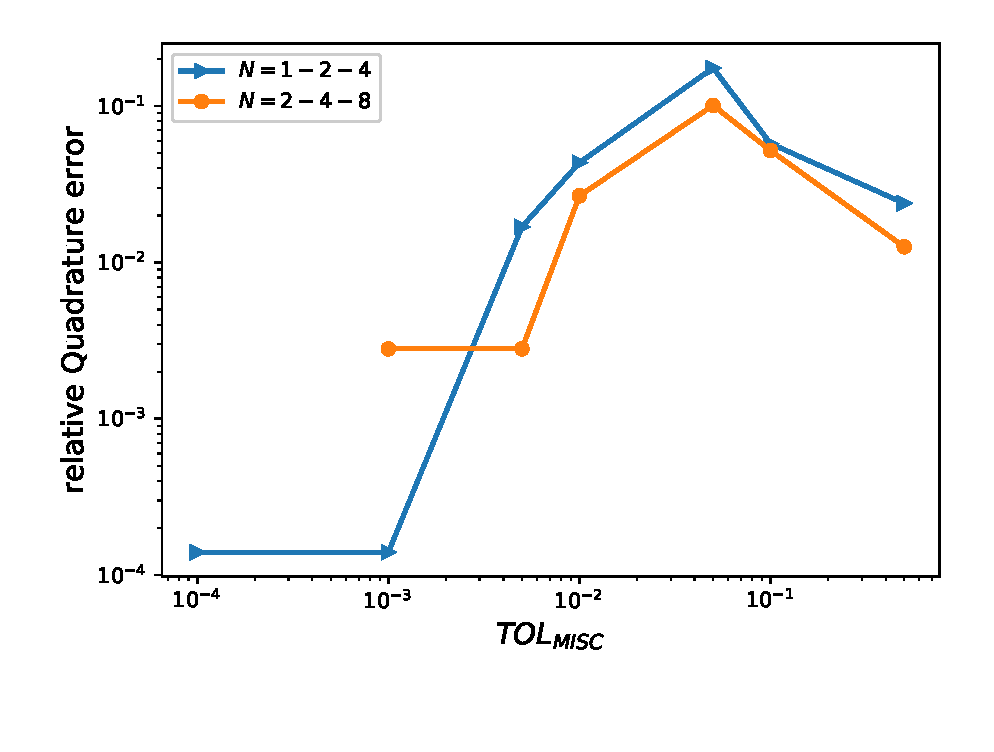
\includegraphics[width=0.5\linewidth]{./figures/rBergomi_MISC_quadratre_error/vs_TOL/set1/relative_quad_error_wrt_MISC_TOL_set1_rich_level2}
	
	
	\caption{Quadrature error of MISC, with different tolerances, to compute call option price of the different tolerances for different number of time steps. Case  set $1$ parameters, with Richardson extrapolation (level $2$).  See detailed values  in table \ref{Quadrature error of MISC to compute Call option price of the different tolerances for different number of time steps. Case set $1$ parameters, with Richardson extrapolation(level $2$). The numbers between parentheses are the corresponding absolute errors.}.}
	\label{fig:Quadrature_error_set1_rich_level2}
\end{figure}




\begin{table}[!h]
	\centering
	\begin{tabular}{l*{6}{c}r}
		Method \textbackslash  Steps            & $1-2-4$ & $2-4-8$  \\
		\hline
%		MISC ($TOL_{\text{MISC}}=5.10^{-1}$)  & $\mathbf{0.1698
%		}$ & $\mathbf{ 0.0150}$  \\
		MISC ($TOL_{\text{MISC}}=10^{-1}$)  & $\mathbf{0.2035
		}$ & $\mathbf{ 0.0544}$ \\
%		MISC ($TOL_{\text{MISC}}=5.10^{-2}$)  & $\mathbf{0.3214
%		}$ & $\mathbf{    0.1035}$  \\
		MISC ($TOL_{\text{MISC}}=10^{-2}$)  & $\mathbf{0.1894}$ & $\mathbf{  0.0291}$   \\	
		MISC ($TOL_{\text{MISC}}=5.10^{-3}$)  & $\mathbf{\red{0.1628}}$ & $\mathbf{\red{0.0052}}$   \\
		MISC ($TOL_{\text{MISC}}=10^{-3}$)  & $\mathbf{0.1460}$ & $\mathbf{0.0052}$   \\
		MISC ($TOL_{\text{MISC}}=10^{-4}$)  & $\mathbf{0.1460}$ & $\mathbf{-}$  \\
		\hline
		MC   & $\mathbf{\red{0.1628}}$  & $\mathbf{\red{0.0052}}$    \\
		\hline
	\end{tabular}
	\caption{Total  relative error of MISC, with different tolerances, and MC to compute call option price for different number of time steps. Case set $1$ parameters in table \ref{table:Reference solution, using MC with $500$ time steps, of Call option price under rBergomi model, for different parameter constellation.}, with Richardson extrapolation(level $2$). The values marked in red, for MISC method, correspond to the total relative errors associated with  stable quadrature errors for MISC, and will be used for complexity comparison against MC.}
	\label{Total  error of MISC and MC to compute Call option price of the different tolerances for different number of time steps. Case set $1$ parameters, with Richardson extrapolation(level $2$). The numbers between parentheses are the corresponding absolute errors.}
\end{table}

\FloatBarrier

\begin{table}[!h]
	\centering
	\begin{tabular}{l*{6}{c}r}
		Method \textbackslash  Steps            & $1-2-4$ & $2-4-8$   \\
		\hline
%		MISC ($TOL_{\text{MISC}}=5.10^{-1}$)  & $0.2$ & $0.3$  \\
		MISC ($TOL_{\text{MISC}}=10^{-1}$)  & $0.25$ & $2$ &   \\
%		MISC ($TOL_{\text{MISC}}=5.10^{-2}$)  & $0.55$ & $5$  \\
		MISC ($TOL_{\text{MISC}}=10^{-2}$)  & $2$ & $24$   \\
		MISC ($TOL_{\text{MISC}}=5.10^{-3}$)  & $\red{5}$ & $\red{64}$  \\	
		MISC ($TOL_{\text{MISC}}=10^{-3}$)  & $24$ & $1067$  \\	
		MISC ($TOL_{\text{MISC}}=10^{-4}$)  & $ 233$ & $-$   \\
		\hline
		MC    & $\red{20}$  & $\red{231}$  \\
		
		\hline
		Ratio of $\left(\text{MC}/ \text{MISC} \right)$  &$\red{4}$ & $\red{  3.6}$   \\
		\hline
	\end{tabular}
	\caption{Comparsion of the computational time (in Seconds) of  MC and MISC, using Richardson extrapolation (level $2$), used to compute call option price of rBergomi model for different number of time steps. Case set $1$ parameters in table \ref{table:Reference solution, using MC with $500$ time steps, of Call option price under rBergomi model, for different parameter constellation.}. The
		average MC CPU time is computed over 10 runs.}
	\label{Comparsion of the computational time of  MC and MISC, using Richardson extrapolation (level $2$), used to compute Call option price of rBergomi model for different number of time steps. Case set $1$ parameters}
\end{table}
















\subsubsection{Case of set $2$ parameters in table \ref{table:Reference solution, using MC with $500$ time steps, of Call option price under rBergomi model, for different parameter constellation.} }
\label{sec:Case of set $2$ parameters_linear}

\subsubsection*{Without Richardson extrapolation}
\begin{table}[h!]
	\centering
	\begin{tabular}{l*{6}{c}r}
		Method \textbackslash  Steps            & $2$ & $4$ & $8$  \\
		\hline
%		MISC ($TOL_{\text{MISC}}=5.10^{-1}$)  & $0.1097$ & $0.0926$ & $0.0807$  \\
		MISC ($TOL_{\text{MISC}}=10^{-1}$)  &$0.1097$ & $0.0926$ & $0.0791$   \\
%		MISC ($TOL_{\text{MISC}}=5.10^{-2}$)  & $0.1097$ & $0.0890$ & $0.0849$  \\
		MISC ($TOL_{\text{MISC}}=10^{-2}$)  & $0.1119$&  $0.1023$ & $0.0910$  \\
		MISC ($TOL_{\text{MISC}}=10^{-3}$)        & $0.1195$ &$0.1023$ &   $0.0910$  \\
		MISC ($TOL_{\text{MISC}}=10^{-4}$)        & $0.1218$ &$0.1023$ &  $-$  \\
		\hline
		MC method ($M=8.10^{6}$)   & $0.1218 $  & $0.1024 $  & $0.0914$  \\		
		\hline
	\end{tabular}
	\caption{ Call option price of the different methods for different number of time steps. Case of set $2$ parameters in table \ref{table:Reference solution, using MC with $500$ time steps, of Call option price under rBergomi model, for different parameter constellation.}, without Richardson extrapolation.}
	\label{table: Call option price of the different methods for different number of time steps. Case set 2_linear}
\end{table}



\begin{table}[h!]
	\centering
	\begin{tabular}{l*{6}{c}r}
		Method \textbackslash  Steps            & $2$ & $4$ & $8$ & $16$  \\
		\hline
		MC Bias ($M=8.10^6$)   & $\underset{(0.0426)}{\mathbf{0.5375
		}}$  & $\underset{ (  0.0208)}{\mathbf{0.2922}}$  & $\underset{(  0.0122)}{\mathbf{0.1542}}$ & $\underset{( 0.0058)}{\mathbf{0.0731}}$  \\	
		
		MC Statistical error ($M=8.10^6$)  & $\underset{( 2.0e-04)}{\mathbf{2.5e-03}}$  & $\underset{(  1.0e-04)}{\mathbf{1.3e-03}}$  & $\underset{(  5.0e-05)}{\mathbf{6.3e-04}}$ & $\underset{(  1.1e-04)}{\mathbf{1.33e-03}}$ \\	
	
		\hline
	\end{tabular}
	\caption{Bias and statistical errors of MC  for computing call option price  for different number of time steps. Case set $2$ parameters in table \ref{table:Reference solution, using MC with $500$ time steps, of Call option price under rBergomi model, for different parameter constellation.}, without Richardson extrapolation. The numbers between parentheses are the corresponding absolute errors.}
	\label{Bias and Statistical errors of MC ($M=10^6$)  for computing Call option price  for different number of time steps. Case set $2$ parameters, without Richardson extrapolation. The numbers between parentheses are the corresponding absolute errors.}
\end{table}





\begin{figure}[h!]
	\centering
	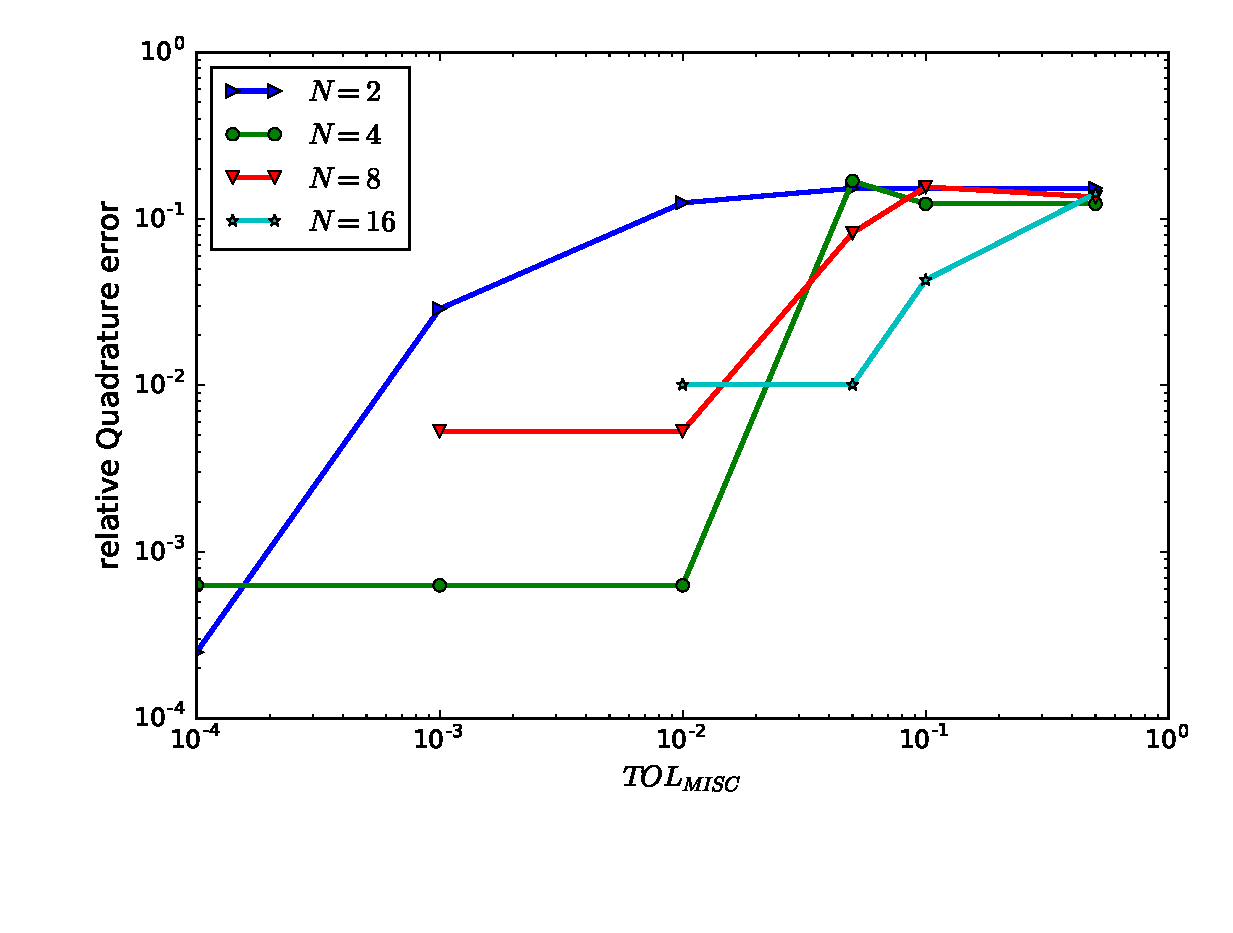
\includegraphics[width=0.5\linewidth]{./figures/rBergomi_MISC_quadratre_error/vs_TOL/set2/relative_quad_error_wrt_MISC_TOL_set2_non_rich_linear}
	
	
	\caption{Quadrature error of MISC, with different tolerances, to compute call option price  of time steps. Case  set $2$ parameters, without Richardson extrapolation.  See detailed values  in table \ref{Quadrature error of MISC to compute Call option price of the different tolerances for different number of time steps. Case  set $2$ parameters, without Richardson extrapolation. The numbers between parentheses are the corresponding absolute errors,linear}.}
	\label{fig:Quadrature_error_set2_linear}
\end{figure}

\FloatBarrier
\begin{table}[h!]
	\centering
	\begin{tabular}{l*{6}{c}r}
		Method \textbackslash  Steps            & $2$ & $4$ & $8$   \\
		\hline
%		MISC ($TOL_{\text{MISC}}=5.10^{-1}$)  & $\mathbf{
%			0.6900}$ & $\mathbf{   
%			0.4153
%		}$ & $\mathbf{    0.2895}$   \\
		MISC ($TOL_{\text{MISC}}=10^{-1}$)  & $\mathbf{
			0.6900}$& $\mathbf{    
			0.4153}$ & $\mathbf{     
			0.3097
		}$   \\
%		MISC ($TOL_{\text{MISC}}=5.10^{-2}$)  &$\mathbf{
%			0.6900}$ & $\mathbf{         0.4608
%		}$ & $\mathbf{      
%			0.2365
%		}$ \\
		MISC ($TOL_{\text{MISC}}=10^{-2}$)  & $\mathbf{ 
			0.6622}$ & $\mathbf{  \red{ 
				0.2928
			}
		}$ & $\mathbf{ \red{    0.1595}}$   \\
		MISC ($TOL_{\text{MISC}}=10^{-3}$)        & $\mathbf{
			0.6371}$  &  $\mathbf{
			0.2928
		}$ &  $\mathbf{    0.1595}$ \\
		MISC ($TOL_{\text{MISC}}=10^{-4}$)        & $\mathbf{       \red{0.5378}}$  & $\mathbf{
			0.2928
		}$  &  $-$ \\
		\hline
		MC    & $\mathbf{\red{    0.5400}}$  & $\mathbf{\red{0.2935}
		}$  &$\mathbf{\red{
				0.1593}}$  \\	
		
		\hline
	\end{tabular}
	\caption{Total relative error of MISC, with different tolerances, and MC to compute Call option price  for different number of time steps. Case  set $2$ parameters in table \ref{table:Reference solution, using MC with $500$ time steps, of Call option price under rBergomi model, for different parameter constellation.}, without Richardson extrapolation. The numbers between parentheses are the corresponding absolute errors. The values marked in red, for MISC method, correspond to the total relative errors associated with  stable quadrature errors for MISC, and will be used for complexity comparison against MC.}
	\label{Total error of MISC and MC to compute Call option price of the different tolerances for different number of time steps. Case $K=1$, $H=0.07$, without Richardson extrapolation. The numbers between parentheses are the corresponding absolute errors,linear}
\end{table}

\begin{table}[h!]
	\centering
	\begin{tabular}{l*{6}{c}r}
		Method \textbackslash  Steps            & $2$ & $4$ & $8$   \\
		\hline
%		MISC ($TOL_{\text{MISC}}=5.10^{-1}$)  & $0.08$ & $0.13$ & $0.2$ \\
		MISC ($TOL_{\text{MISC}}=10^{-1}$)  & $0.08$ & $0.13$ & $0.7$   \\
%		MISC ($TOL_{\text{MISC}}=5.10^{-2}$)  & $0.08$ & $0.25$ & $7$   \\
		MISC ($TOL_{\text{MISC}}=10^{-2}$)  & $0.2$& $\red{5}$ & $\red{333}$   \\
		MISC ($TOL_{\text{MISC}}=10^{-3}$)  &  $2$ & $73$ & $3650$  \\		
		MISC ($TOL_{\text{MISC}}=10^{-4}$)  & $\red{43}$ & $1240$ & $-$  \\	
	
		\hline
		MC method & $\red{220}$  & $\red{358}$  & $\red{9}$  \\
		\hline	
		Ratio of $\left(\text{MC}/ \text{MISC} \right)$  &$\red{5}$ & $\red{   72 
		}$  & $\red {  0.03	}$   \\
		\hline
	\end{tabular}
	\caption{Comparison of the computational time (in Seconds) of  MC and MISC, used to compute Call option price of rBergomi model for different number of time steps. Case  set $2$ parameters in table \ref{table:Reference solution, using MC with $500$ time steps, of Call option price under rBergomi model, for different parameter constellation.}. The
		average MC CPU time is computed over 10 runs.}
	\label{Comparsion of the computational time of  MC and MISC, used to compute Call option price of rBergomi model for different number of time steps. Case $K=1, H=0.07$, linear}
\end{table}

\FloatBarrier
\subsubsection*{With Richardson extrapolation (level $1$)}

\begin{table}[h!]
	\centering
	\begin{tabular}{l*{6}{c}r}
		Method \textbackslash  Steps    &$1-2$         & $2-4$ & $4-8$ \\
		\hline
%		MISC ($TOL_{\text{MISC}}=5.10^{-1}$)  &$0.1260$ & $0.0756$ & $0.0687$\\
		MISC ($TOL_{\text{MISC}}=10^{-1}$)  &$0.1260$ & $0.0756$ & $0.0702$   \\
		MISC ($TOL_{\text{MISC}}=5.10^{-2}$)   &$0.1260$ & $0.0716$ & $0.0796$    \\
		MISC ($TOL_{\text{MISC}}=10^{-2}$)  &$0.1456$ & $0.0838$ & $0.0796$  \\	
		MISC ($TOL_{\text{MISC}}=10^{-3}$)  &$0.1497$ & $0.0838$ & $-$ \\
		
		MISC ($TOL_{\text{MISC}}=10^{-4}$)  &$0.1501$ & $-$ & $-$ \\
		\hline
		MC method ($M=10^{6}$)   & $0.1552 $  & $0.0846 $  & $0.0804$  \\		
		\hline
	\end{tabular}
	\caption{Call option price of the different methods for different number of time steps. Case set $2$ parameters of table \ref{table:Reference solution, using MC with $500$ time steps, of Call option price under rBergomi model, for different parameter constellation.}, using Richardson extrapolation (level $1$)}
	\label{table:  Call option price of the different methods for different number of time steps. Case set $2$ parameter, using Richardson extrapolation (level $1$),linear}
\end{table}



\begin{table}[h!]
	\centering
	\begin{tabular}{l*{6}{c}r}
		Method \textbackslash  Steps            & $1-2$ & $2-4$ & $4-8$ & $8-16$  \\
		\hline
		MC Bias ($M=10^6$)  &$\underset{( 0.0760)}{\mathbf{0.9594}}$  & $\underset{( 0.0054)}{\mathbf{0.0686}}$  & $\underset{(   0.0012)}{\mathbf{0.0149}}$  & $\underset{(  0.0004)}{\mathbf{0.0048}}$ \\	
		
		MC Statistical error ($M=10^6$)   & $\underset{( 1e-03)}{\mathbf{1.3e-02}}$  & $\underset{(   3.2e-04)}{\mathbf{4.1e-03}}$  & $\underset{(  1.7e-04)}{\mathbf{2.1e-03}}$ & $\underset{(  1.3e-04)}{\mathbf{1.6e-03}}$ \\	
		\hline
	\end{tabular}
	\caption{Bias and statistical errors of MC   for computing call option price  for different number of time steps. Case set $2$ parameters in tabel \ref{table:Reference solution, using MC with $500$ time steps, of Call option price under rBergomi model, for different parameter constellation.}, with Richardson extrapolation (level $1$). The numbers between parentheses are the corresponding absolute errors.}
	\label{Bias and Statistical errors of MC ($M=10^6$)  for computing Call option price  for different number of time steps. Case set $2$ parameters, with Richardson extrapolation (level1). The numbers between parentheses are the corresponding absolute errors.}
\end{table}








\begin{figure}[h!]
	\centering
	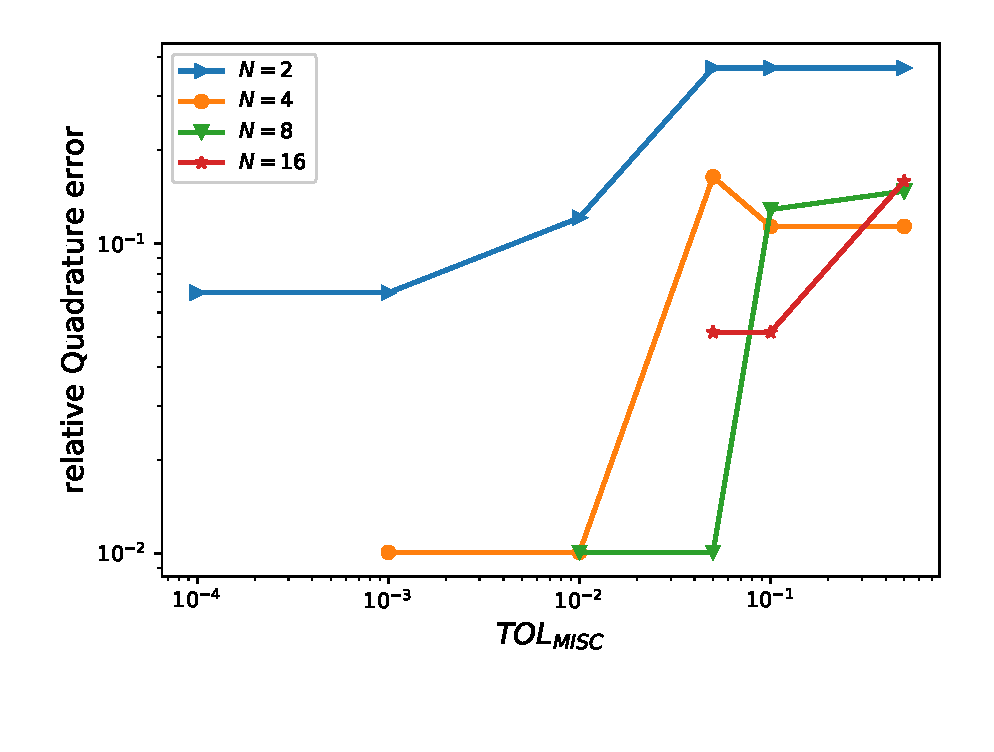
\includegraphics[width=0.5\linewidth]{./figures/rBergomi_MISC_quadratre_error/vs_TOL/set2/relative_quad_error_wrt_MISC_TOL_set2_with_rich_linear}
	
	
	\caption{Quadrature error of MISC, with different tolerances,  to compute call option price for different number of time steps. Case  set $2$ parameters, with Richardson extrapolation.  See detailed values  in table \ref{Quadrature error of MISC to compute Call option price of the different tolerances for different number of time steps. Case set $2$ parameters, with Richardson extrapolation(level $1$). The numbers between parentheses are the corresponding absolute errors,linear}.}
	\label{fig:Quadrature_error_set2_linear_rich}
\end{figure}


\begin{table}[h!]
	\centering
	\begin{tabular}{l*{6}{c}r}
		Method \textbackslash  Steps            & $1-2$ & $2-4$ & $4-8$  \\
		\hline
%		MISC ($TOL_{\text{MISC}}=5.10^{-1}$)  & $\mathbf{  1.3281}$ & $\mathbf{  0.1822}$ & $\mathbf{
%			0.1626
%		}$  \\
		MISC ($TOL_{\text{MISC}}=10^{-1}$)  & $\mathbf{  1.3281}$ & $\mathbf{0.1822}$ & $\mathbf{0.1437}$   \\
		MISC ($TOL_{\text{MISC}}=5.10^{-2}$)  & $\mathbf{  1.3281}$ & $\mathbf{ 0.2327}$ & $\mathbf{  \red{0.0250}}$   \\
		MISC ($TOL_{\text{MISC}}=10^{-2}$)  & $\mathbf{   1.0806
		}$ & $\mathbf{    \red{0.0787}}$ & $\mathbf{ 0.0250}$  \\
		MISC ($TOL_{\text{MISC}}=10^{-3}$)  & $\mathbf{ \red{  1.0288}}$ & $\mathbf{    0.0787}$ & $\mathbf{-}$  \\
		
		MISC ($TOL_{\text{MISC}}=10^{-4}$)  & $\mathbf{     1.0238}$ & $\mathbf{-}$ & $\mathbf{-}$  \\

		\hline
		
		MC &$\mathbf{ \red{  1.0288}}$  & $\mathbf{\red{0.0787}}$ & $\mathbf{\red{0.0250}}$  \\
		
		\hline
	\end{tabular}
	\caption{Total relative error of MISC, with different tolerances,  and MC to compute call option price  for different number of time steps. Case set $2$ parameters in table \ref{table:Reference solution, using MC with $500$ time steps, of Call option price under rBergomi model, for different parameter constellation.}, with Richardson extrapolation(level $1$). The numbers between parentheses are the corresponding absolute errors. The values marked in red, for MISC method, correspond to the total relative errors associated with  stable quadrature errors for MISC, and will be used for complexity comparison against MC.}
	\label{Total  error of MISC and MC to compute Call option price of the different tolerances for different number of time steps. Case set $2$ parameters, with Richardson extrapolation(level $1$). The numbers between parentheses are the corresponding absolute errors,relative}
\end{table}


\begin{table}[h!]
	\centering
	\begin{tabular}{l*{6}{c}r}
		Method \textbackslash  Steps            & $1-2$ & $2-4$ & $4-8$   \\
		\hline
%		MISC ($TOL_{\text{MISC}}=5.10^{-1}$)  & $0.1$ & $0.18$ & $0.3$   \\
		MISC ($TOL_{\text{MISC}}=10^{-1}$)  & $0.1$ & $0.18$ & $1.6$  \\
		MISC ($TOL_{\text{MISC}}=5.10^{-2}$)  & $0.1$ & $0.6$ & $\red{37}$  \\
		MISC ($TOL_{\text{MISC}}=10^{-2}$)  & $1.3$ & $\red{6}$ & $2382$  \\
		MISC ($TOL_{\text{MISC}}=10^{-3}$)  & $\red{3.5}$ & $ 244$ & $-$   \\
		
		MISC ($TOL_{\text{MISC}}=10^{-4}$)  & $140$ & $-$ & $-$ \\
		\hline	
		MC  &$\red{12}$ & $\red{113}$  & $\red{130}$   \\
		
		\hline	
		Ratio of $\left(\text{MC}/ \text{MISC} \right)$  &$\red{ 3.4
		}$ & $\red{     18.8
		}$  & $\red{ 3.5}
		$  \\
		\hline
		\end{tabular}
		\caption{Comparison of the computational time (in Seconds) of  MC and MISC, using Richardson extrapolation (level $1$), used to compute call option price of rBergomi model for different number of time steps. Case set $2$ parameters in table \ref{table:Reference solution, using MC with $500$ time steps, of Call option price under rBergomi model, for different parameter constellation.}. The
			average MC CPU time is computed over 10 runs.}
		\label{Comparsion of the computational time of  MC and MISC, using Richardson extrapolation (level $1$), used to compute Call option price of rBergomi model for different number of time steps. Case set $2$ parameters,linear}
		\end{table}
		
		\FloatBarrier
	\subsubsection*{With Richardson extrapolation (level $2$)}
		

		\begin{table}[h!]
		\centering
		\begin{tabular}{l*{6}{c}r}
		Method \textbackslash  Steps           &$1-2-4$ & $2-4-8$ \\
		\hline
%		MISC ($TOL_{\text{MISC}}=5.10^{-1}$)& $0.0587$  & $0.0664 $ \\
		
		MISC ($TOL_{\text{MISC}}=10^{-1}$)  &$0.0587$  &$ 0.0702$   \\
		MISC ($TOL_{\text{MISC}}=5.10^{-2}$)  & $0.0401$ & $0.0790$  \\
		MISC ($TOL_{\text{MISC}}=10^{-2}$)  & $0.0623$ &  $0.0784$   \\
		MISC ($TOL_{\text{MISC}}=5.10^{-3}$)  & $0.0623$ & $-$   \\
		MISC ($TOL_{\text{MISC}}=10^{-3}$)  & $0.0608$ & $$  \\
		
		\hline
		MC ($M=3.10^6$)  & $ 0.0601$ & $ 0.0787$   \\
		\hline 
	\end{tabular}
	\caption{ Call option price of the different methods for different number of time steps. Case set $2$ parameters in tabel \ref{table:Reference solution, using MC with $500$ time steps, of Call option price under rBergomi model, for different parameter constellation.}, using Richardson extrapolation (level 2).}
	\label{table: Call option price of the different methods for different number of time steps. Case $K=1,H=0.07$, using Richardson extrapolation_level2,linear}
\end{table}




\begin{table}[h!]
	\centering
	\begin{tabular}{l*{6}{c}r}
		Method \textbackslash  Steps            & $1-2-4$ & $2-4-8$  \\
		\hline
		MC  Bias  ($M=3.10^6$)   &$\underset{(  0.0191)}{\mathbf{  0.2411}}$  & $\underset{(      4.6e-04)}{\mathbf{  0.0058}}$   \\	
		
		MC Statistical error ($M=3.10^6$)   & $\underset{( 2.8e-04)}{\mathbf{3.5e-03}}$  & $\underset{(   1.4e-04)}{\mathbf{    1.8e-03}}$  \\	
		
		
		
		\hline
	\end{tabular}
	\caption{Bias and statistical errors of MC   for computing call option price  for different number of time steps. Case set $2$ parameters in tabel \ref{table:Reference solution, using MC with $500$ time steps, of Call option price under rBergomi model, for different parameter constellation.}, with Richardson extrapolation (level $2$). The numbers between parentheses are the corresponding absolute errors.}
	\label{Bias and Statistical errors of MC ($M=3.10^6$)  for computing Call option price  for different number of time steps. Case set $2$ parameters, with Richardson extrapolation (level2). The numbers between parentheses are the corresponding absolute errors.}
\end{table}





\begin{figure}[h!]
	\centering
	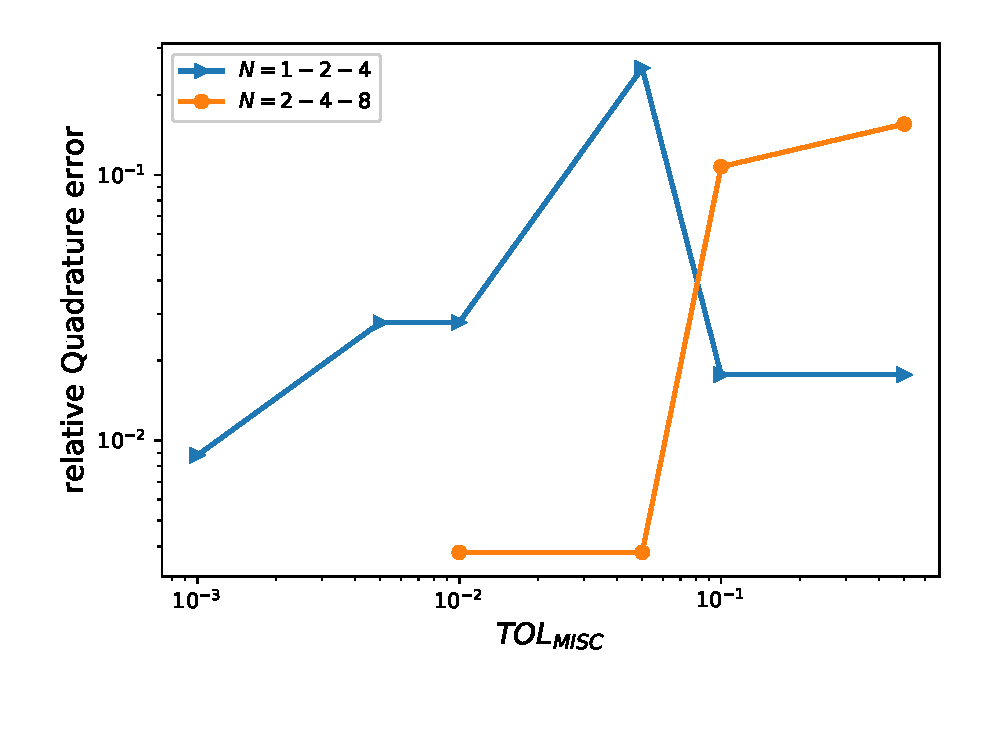
\includegraphics[width=0.5\linewidth]{./figures/rBergomi_MISC_quadratre_error/vs_TOL/set2/relative_quad_error_wrt_MISC_TOL_set2_rich_level2_linear}
	
	
	\caption{Quadrature error of MISC to compute Call option price of the different tolerances for different number of time steps. Case  set $2$ parameters, with Richardson extrapolation (level $2$).  See detailed values  in table \ref{Quadrature error of MISC to compute Call option price of the different tolerances for different number of time steps. Case set $2$ parameters, with Richardson extrapolation(level $2$). The numbers between parentheses are the corresponding absolute errors,linear}.}
	\label{fig:Quadrature_error_set2_rich_linear}
\end{figure}


\begin{table}[!h]
	\centering
	\begin{tabular}{l*{6}{c}r}
		Method \textbackslash  Steps            & $1-2-4$ & $2-4-8$  \\
		\hline
%		MISC ($TOL_{\text{MISC}}=5.10^{-1}$)  & $\mathbf{ 0.2588
%		}$ & $\mathbf{ 0.1611}$  \\
		MISC ($TOL_{\text{MISC}}=10^{-1}$)  & $\mathbf{ 0.2588
		}$ & $\mathbf{ 0.1131}$ \\
		MISC ($TOL_{\text{MISC}}=5.10^{-2}$)  & $\mathbf{   0.4936
		}$ & $\mathbf{\red{ 0.0096} }$  \\
		MISC ($TOL_{\text{MISC}}=10^{-2}$)  & $\mathbf{ \red{0.2689}}$ & $\mathbf{ 0.0096 }$    \\	
		MISC ($TOL_{\text{MISC}}=5.10^{-3}$)  & $\mathbf{ 0.2689}$ & $\mathbf{-}$   \\
		MISC ($TOL_{\text{MISC}}=10^{-3}$)  & $\mathbf{ 0.2499}$ & $\mathbf{-}$   \\
		\hline
		MC   & $\mathbf{\red{0.2689}}$  & $\mathbf{\red{ 0.0096}}$    \\
		\hline
	\end{tabular}
	\caption{Total relative  error of MISC, with different tolerances, and MC to compute call option price   for different number of time steps. Case set $2$ parameters in table \ref{table:Reference solution, using MC with $500$ time steps, of Call option price under rBergomi model, for different parameter constellation.}, with Richardson extrapolation(level $2$). The values marked in red, for MISC method, correspond to the total relative errors associated with  stable quadrature errors for MISC, and will be used for complexity comparison against MC.}
	\label{Total  error of MISC and MC to compute Call option price of the different tolerances for different number of time steps. Case set $2$ parameters, with Richardson extrapolation(level $2$). The numbers between parentheses are the corresponding absolute errors,linear}
\end{table}

\begin{table}[!h]
	\centering
	\begin{tabular}{l*{6}{c}r}
		Method \textbackslash  Steps            & $1-2-4$ & $2-4-8$   \\
		\hline
%		MISC ($TOL_{\text{MISC}}=5.10^{-1}$)  & $0.2$ & $0.4$  \\
		MISC ($TOL_{\text{MISC}}=10^{-1}$)  & $0.2$ & $2$ &   \\
		MISC ($TOL_{\text{MISC}}=5.10^{-2}$)  & $0.5$ & $\red{74}$  \\
		MISC ($TOL_{\text{MISC}}=10^{-2}$)  & $\red{9}$ & $3455$   \\
		MISC ($TOL_{\text{MISC}}=5.10^{-3}$)  & $30$ & $-$  \\	
		MISC ($TOL_{\text{MISC}}=10^{-3}$)  & $693$ & $-$  \\	
		\hline
		MC    & $ \red{  118}$  & $\red{1274}$  \\
		
		\hline
		Ratio of $\left(\text{MC}/ \text{MISC} \right)$  &$\red{13}$ & $\red{  17}$   \\
		\hline
	\end{tabular}
	\caption{Comparison of the computational time (in Seconds) of  MC and MISC, using Richardson extrapolation (level $2$), used to compute call option price of rBergomi model for different number of time steps. Case set $2$ parameters in table \ref{table:Reference solution, using MC with $500$ time steps, of Call option price under rBergomi model, for different parameter constellation.}. The
		average MC CPU time is computed over 10 runs.}
	\label{Comparsion of the computational time of  MC and MISC, using Richardson extrapolation (level $2$), used to compute Call option price of rBergomi model for different number of time steps. Case set $2$ parameters,linear}
\end{table}





\FloatBarrier

\subsubsection{Case of set $3$ parameters in table \ref{table:Reference solution, using MC with $500$ time steps, of Call option price under rBergomi model, for different parameter constellation.}}\label{sec:Case of set 3 parameters}


\subsubsection*{Without Richardson extrapolation}

\begin{table}[h!]
	\centering
	\begin{tabular}{l*{6}{c}r}
		Method \textbackslash  Steps            & $2$ & $4$ & $8$ & $16$ &   \\
		\hline
%		MISC ($TOL_{\text{MISC}}=5.10^{-1}$)  & $0.1258$ & $0.1239$ & $0.1231$ & $0.1227$  \\
		MISC ($TOL_{\text{MISC}}=10^{-1}$)  & $0.1258$ & $0.1239$ & $0.1231$ & $0.1229$  \\
%		MISC ($TOL_{\text{MISC}}=5.10^{-2}$)  & $0.1258$ & $0.1239$ & $0.1231$ & $0.1241$  \\
		MISC ($TOL_{\text{MISC}}=10^{-2}$)  & $0.1258$ & $0.1246$ & $0.1248$ & $0.1250$  \\
		
		MISC ($TOL_{\text{MISC}}=10^{-3}$)  & $0.1271$ & $0.1259$ & $0.1252$ & $0.1249$  \\
		MISC ($TOL_{\text{MISC}}=10^{-4}$)  & $0.1270$ & $0.1258$ & $0.1252$ & $-$  \\
		
			MISC ($TOL_{\text{MISC}}=10^{-5}$)  & $0.1270$ &$0.1258$ &  $0.1252$ & $-$  \\
		\hline
		MC method ($M=3.10^{6}$)   & $    0.1269$ & $0.1257$  & $0.1253$ & $0.1249$ \\		
		
		\hline
	\end{tabular}
	\caption{ Call option price of the different methods for different number of time steps. Case of set $3$ parameters in table \ref{table:Reference solution, using MC with $500$ time steps, of Call option price under rBergomi model, for different parameter constellation.}, without Richardson extrapolation.}
	\label{table: Call option price of the different methods for different number of time steps. Case set 3}
\end{table}


\begin{table}[h!]
	\centering
	\begin{tabular}{l*{6}{c}r}
		Method \textbackslash  Steps            & $2$ & $4$ & $8$ & $16$  \\
		\hline
		MC Bias ($M=3.10^6$)   & 	$ \underset{(    0.0022)}{\mathbf{0.0174}}$  & $\underset{(0.001)}{\mathbf{0.0078}}$  & $\underset{(0.0005)}{\mathbf{0.0042}}$ & $\underset{(0.0001)}{\mathbf{0.0008}}$\\ 
		
		MC Statistical error ($M=3.10^6$)  &  $\underset{(   6.2e-05)} {\mathbf{5.0e-04}}$  & $\underset{(5.9e-05)} {\mathbf{4.7e-04}}$  & $\underset{(5.8e-05)} {\mathbf{4.6e-04 }}$ & $\underset{(5.8e-05)} {\mathbf{4.6e-04 }}$	\\
		
		\hline
	\end{tabular}
	\caption{Bias and statistical errors of MC   for computing call option price  for different number of time steps. Case set $3$, without Richardson extrapolation. The numbers between parentheses are the corresponding absolute errors.}
	\label{Bias and Statistical errors of MC ($M=10^6$)  for computing Call option price  for different number of time steps. Case set 3, without Richardson extrapolation. The numbers between parentheses are the corresponding absolute errors.}
\end{table}






	\begin{figure}[h!]
		\centering
		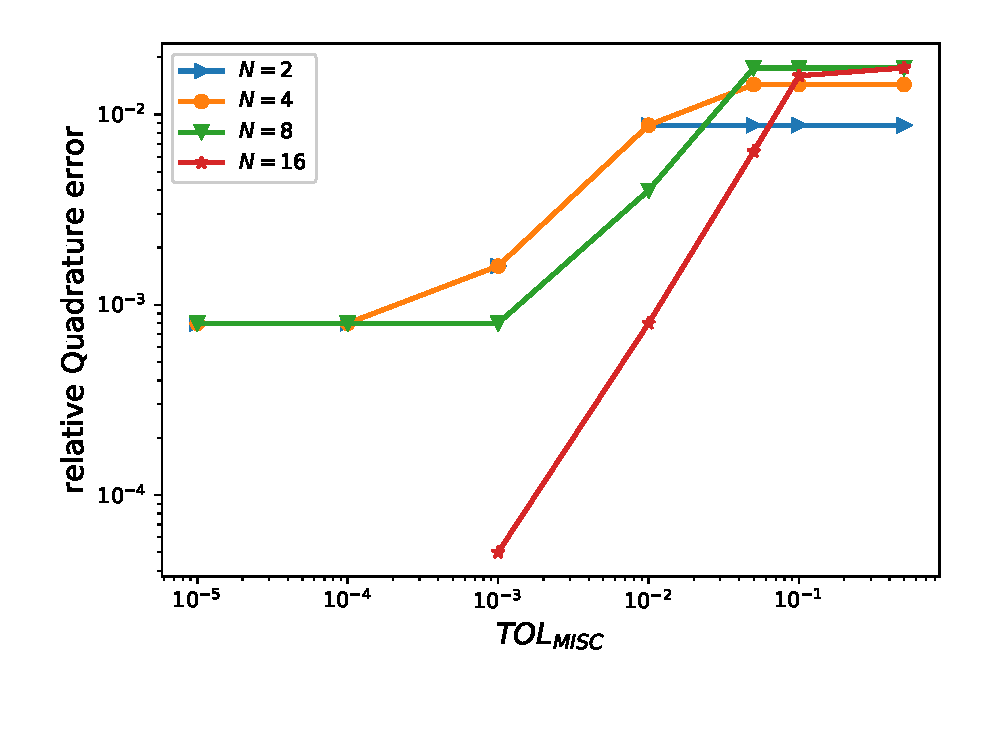
\includegraphics[width=0.5\linewidth]{./figures/rBergomi_MISC_quadratre_error/vs_TOL/set5/relative_quad_error_wrt_MISC_TOL_set5_non_rich}
	
	
	\caption{Quadrature error of MISC, with different tolerances, to compute call option price  for different number of time steps. Case  set $3$ parameters, without Richardson extrapolation.  See detailed values  in table \ref{Quadrature error of MISC to compute Call option price of the different tolerances for different number of time steps. Case  set $3$ parameters, without Richardson extrapolation. The numbers between parentheses are the corresponding absolute errors.}.}
	\label{fig:Quadrature_error_set3}
\end{figure}




\begin{table}[h!]
	\centering
	\begin{tabular}{l*{6}{c}r}
		Method \textbackslash  Steps            & $2$ & $4$ & $8$ & $16$  \\
		\hline
%		MISC ($TOL_{\text{MISC}}=5.10^{-1}$)  & $\mathbf{0.0262}$ & $\mathbf{0.0222}$ & $\mathbf{ 0.0218}$ & $\mathbf{ 0.0184}$  \\
		MISC ($TOL_{\text{MISC}}=10^{-1}$)  &  $\mathbf{0.0262}$ & $\mathbf{0.0222}$& $\mathbf{ 0.0218}$ & $\mathbf{ 0.0168}$   \\
%		MISC ($TOL_{\text{MISC}}=5.10^{-2}$)  & $\mathbf{0.0262}$ & $\mathbf{0.0222}$ & $\mathbf{ 0.0218}$ & $\mathbf{ 0.0072}$  \\
		MISC ($TOL_{\text{MISC}}=10^{-2}$)  &  $\mathbf{0.0262}$ & $\mathbf{0.0166}$& $\mathbf{ 0.0082}$ & $\mathbf{ \red{0.0016}}$  \\
		MISC ($TOL_{\text{MISC}}=10^{-3}$)  &  $\mathbf{0.0190}$ & $\mathbf{0.0094}$& $\mathbf{\red{0.0050}}$  & $\mathbf{ 0.0008}$  \\
		MISC ($TOL_{\text{MISC}}=10^{-4}$)  &  $\mathbf{\red{0.0182}}$ & $\mathbf{\red{0.0086}}$& $\mathbf{0.0050}$ & $\mathbf{ -}$ \\
			MISC ($TOL_{\text{MISC}}=10^{-5}$)  &  $\mathbf{0.0182}$ & $\mathbf{0.0086}$& $\mathbf{0.0050}$ & $\mathbf{ -}$ 
			 \\
		\hline
		MC    & $\mathbf{\red{0.0179}}$  & $\mathbf{ \red{0.0083}}$  & $\mathbf{\red{0.0047}}$ & $\mathbf{ \red{0.0013}}$  \\		
		\hline
	\end{tabular}
	\caption{Total relative error of MISC, with different tolerances, and MC to compute call option price for different number of time steps. Case set $3$ parametrs of table \ref{table:Reference solution, using MC with $500$ time steps, of Call option price under rBergomi model, for different parameter constellation.}, without Richardson extrapolation. The numbers between parentheses are the corresponding absolute errors. The values marked in red, for MISC method, correspond to the total relative errors associated with  stable quadrature errors for MISC, and will be used for complexity comparison against MC.}
	\label{Total error of MISC and MC to compute Call option price of the different tolerances for different number of time steps. Case set 3, without Richardson extrapolation. The numbers between parentheses are the corresponding absolute errors.}
\end{table}



\begin{table}[h!]
	\centering
	\begin{tabular}{l*{6}{c}r}
		Method \textbackslash  Steps            & $2$ & $4$ & $8$ & $16$ &   \\
		\hline
%		MISC ($TOL_{\text{MISC}}=5.10^{-1}$)  & $0.1$ & $0.1$ & $0.2$ & $0.4$  \\
		MISC ($TOL_{\text{MISC}}=10^{-1}$)  & $0.1$ & $0.1$ & $0.2$ & $0.8$ \\
%		MISC ($TOL_{\text{MISC}}=5.10^{-2}$)  & $0.1$ & $0.1$ & $0.2$ & $22$  \\
		MISC ($TOL_{\text{MISC}}=10^{-2}$)  & $0.1$ & $0.5$ & $8$ & $\red{92}$ \\
		MISC ($TOL_{\text{MISC}}=10^{-3}$)  & $0.5$ & $3$ & $\red{24}$ & $2226$ \\
		MISC ($TOL_{\text{MISC}}=10^{-4}$)  & $\red{1}$ & $\red{6}$ & $80$ & $-$\\
		MISC ($TOL_{\text{MISC}}=10^{-5}$)  & $2$ & $32$ & $1760$ & $-$
		 \\
		\hline
		MC method   & $ \red{122}
		
		$  & $  \red{211}$  & $  \red{427}$ & $ \red{766}
		$  \\	
		\hline
		Ratio of $\left(MC/MISC \right)$ & $ \red{122}
		
		$  & $  \red{35}$  & $  \red{  18
		}$ & $ \red{ 8}
		$  \\	
		
		\hline
	\end{tabular}
	\caption{Comparison of the computational time (in Seconds) of  MC and MISC, used to compute Call option price of rBergomi model for different number of time steps. Case set $3$ parametrs of table \ref{table:Reference solution, using MC with $500$ time steps, of Call option price under rBergomi model, for different parameter constellation.}. The average  MC CPU time is computed over $10$ runs. }
	\label{Comparsion of the computational time of  MC and MISC, used to compute Call option price of rBergomi model for different number of time steps. Case set3}
\end{table}

	\begin{figure}[h!]
	\centering
	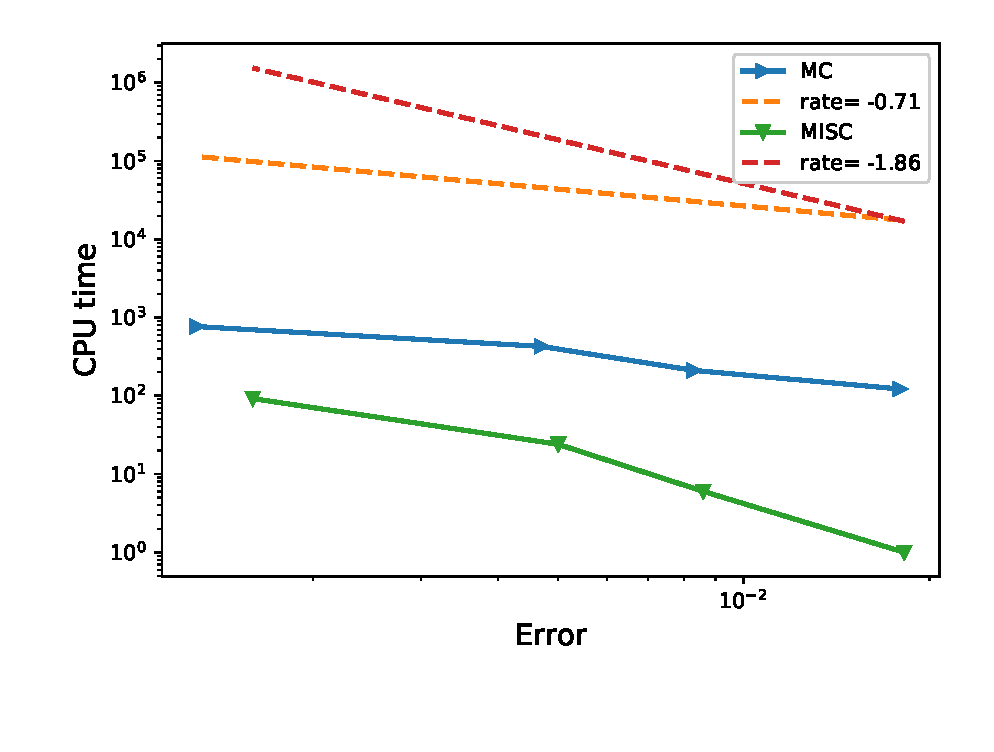
\includegraphics[width=0.5\linewidth]{./figures/rBergomi_Complexity_rates/set5/error_vs_time_set5}

	\caption{Complexity plot for   MC and MISC for case set $3$ parameters of table \ref{table:Reference solution, using MC with $500$ time steps, of Call option price under rBergomi model, for different parameter constellation.}.}
	\label{fig:Complexity plot for MC and MISC for Case set $3$ parameters}
\end{figure}



\FloatBarrier
\subsubsection*{With Richardson extrapolation (level $1$)}
\begin{table}[h!]
	\centering
	\begin{tabular}{l*{6}{c}r}
		Method \textbackslash  Steps    &$1-2$         & $2-4$ & $4-8$ & $8-16$\\
		\hline
%		MISC ($TOL_{\text{MISC}}=5.10^{-1}$)   &$ 0.1261$ & $0.1220$ & $0.1222$ & $0.1223$\\
		MISC ($TOL_{\text{MISC}}=10^{-1}$)   &$ 0.1261$ & $0.1220$  &$0.1222$ & $0.1226$\\
%		MISC ($TOL_{\text{MISC}}=5.10^{-2}$)   &$ 0.1261$ & $0.1220$  & $0.1222$ & $0.1240$ \\
		MISC ($TOL_{\text{MISC}}=10^{-2}$)   &$ 0.1267$ & $0.1230$ & $0.1245$ & $0.1247$  \\	
		MISC ($TOL_{\text{MISC}}=10^{-3}$)   &$0.1285$ & $0.1247$ & $0.1247$ &  $0.1247$ \\
		MISC ($TOL_{\text{MISC}}=10^{-4}$)  &$0.1285$ & $0.1247$ & $0.1247$ & $-$ \\
			MISC ($TOL_{\text{MISC}}=10^{-5}$)  &$0.1285$ & $0.1247$ &  $0.1247$ & $-$ \\
	
		\hline
		MC method ($M=10^{7}$)   & $     0.1284$  & $ 
		0.1251$  & $0.1249$ & $  0.1248$ \\		
		\hline
	\end{tabular}
	\caption{Call option price of the different methods for different number of time steps. Case set $3$ parameters of table \ref{table:Reference solution, using MC with $500$ time steps, of Call option price under rBergomi model, for different parameter constellation.}, using Richardson extrapolation (level $1$).}
	\label{table:  Call option price of the different methods for different number of time steps. Case set $5$ parameter, using Richardson extrapolation (level $3$)}
\end{table}



\begin{table}[h!]
	\centering
	\begin{tabular}{l*{6}{c}r}
		Method \textbackslash  Steps            & $1-2$ & $2-4$ & $4-8$ & $8-16$  \\
		\hline
		MC Bias ($M=10^7$)  &$\underset{(  0.0037
			)}{\mathbf{0.0295}}$  & $\underset{( 0.0003)}{\mathbf{0.0025}}$  & $\underset{(   0.0001)}{\mathbf{0.0009}}$  & $\underset{(  6.2e-05)}{\mathbf{0.0005}}$ \\	
		
		MC Statistical error ($M=10^7$)   & $\underset{(  4.4e-05)}{\mathbf{3.5e-04}}$  & $\underset{(   4.2e-05)}{\mathbf{3.4e-04}}$  & $\underset{(  4.1e-05)}{\mathbf{3.3e-04}}$ & $\underset{(  4.1e-05)}{\mathbf{3.3e-04}}$ \\	
	
		\hline
	\end{tabular}
	\caption{Bias and statistical errors of MC   for computing call option price  for different number of time steps. Case set $3$ parameters in tabel \ref{table:Reference solution, using MC with $500$ time steps, of Call option price under rBergomi model, for different parameter constellation.}, with Richardson extrapolation (level $1$). The numbers between parentheses are the corresponding absolute errors.}
	\label{Bias and Statistical errors of MC ($M=10^7$)  for computing Call option price  for different number of time steps. Case set $3$ parameters, with Richardson extrapolation (level1). The numbers between parentheses are the corresponding absolute errors.}
\end{table}








\begin{figure}[h!]
	\centering
	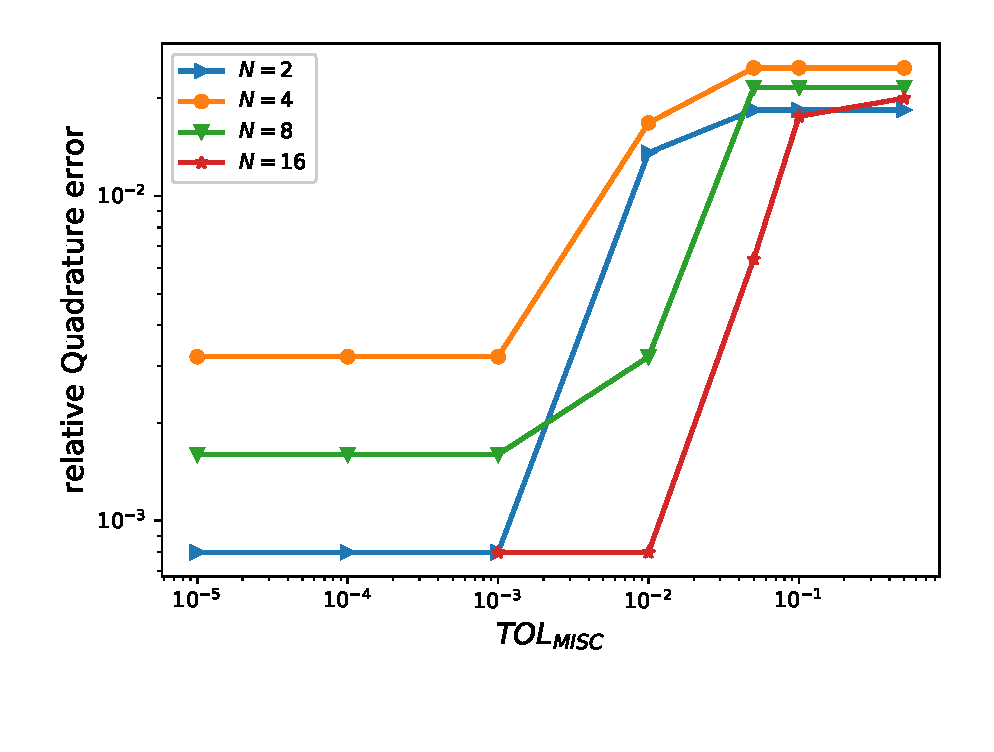
\includegraphics[width=0.5\linewidth]{./figures/rBergomi_MISC_quadratre_error/vs_TOL/set5/relative_quad_error_wrt_MISC_TOL_set5_with_rich}
	
	
	\caption{Quadrature error of MISC, with  different tolerances,  to compute call option price, for different number of time steps. Case  set $3$ parameters, with Richardson extrapolation.  See detailed values  in table \ref{Quadrature error of MISC to compute Call option price of the different tolerances for different number of time steps. Case set $3$ parameters, with Richardson extrapolation(level $1$). The numbers between parentheses are the corresponding absolute errors.}.}
	\label{fig:Quadrature_error_set3_rich}
\end{figure}

\begin{table}[h!]
	\centering
	\begin{tabular}{l*{6}{c}r}
		Method \textbackslash  Steps           & $2-4$ & $4-8$ & $8-16$  \\
		\hline
%		MISC ($TOL_{\text{MISC}}=5.10^{-1}$)  & $0.0273$  & $0.0225$ & $0.0205$  \\
		MISC ($TOL_{\text{MISC}}=10^{-1}$)  &$0.0273$  &$0.0225$ & $0.0181$  \\
%		MISC ($TOL_{\text{MISC}}=5.10^{-2}$)  & $0.0273$  &$0.0225$ & $0.0069$  \\
			MISC ($TOL_{\text{MISC}}=10^{-2}$)  & $0.0193$  & $0.0041$ & $\red{0.0013}$  \\
		MISC ($TOL_{\text{MISC}}=10^{-3}$)  & $\red{0.0057}$  & $\red{0.0025}$ & $0.0013$  \\
		MISC ($TOL_{\text{MISC}}=10^{-4}$)    &$0.0057$  & $0.0033$  & $-$  \\
			MISC ($TOL_{\text{MISC}}=10^{-5}$)    &$0.0057$   &  $0.0033$ & $-$  \\	
	\hline

		MC    & $\red{\mathbf{0.0073}}$  &   $\red{\mathbf{0.0025}}$  &  $\red{\mathbf{0.0013}}$  \\
		\hline
	\end{tabular}
	\caption{Total relative error of MISC, with different tolerances, and MC to compute Call option price  for different number of time steps. Case set $3$ parameters in table \ref{table:Reference solution, using MC with $500$ time steps, of Call option price under rBergomi model, for different parameter constellation.}, with Richardson extrapolation(level $1$). The numbers between parentheses are the corresponding absolute errors. The values marked in red, for MISC method, correspond to the total relative errors associated with  stable quadrature errors for MISC, and will be used for complexity comparison against MC.}
	\label{Total  error of MISC and MC to compute Call option price of the different tolerances for different number of time steps. Case set $3$ parameters, with Richardson extrapolation(level $1$). The numbers between parentheses are the corresponding absolute errors.}
\end{table}



\begin{table}[h!]
	\centering
	\begin{tabular}{l*{6}{c}r}
		Method \textbackslash  Steps            & $2-4$ & $4-8$ & $8-16$ &   \\
		\hline
%		MISC ($TOL_{\text{MISC}}=5.10^{-1}$)    & $0.15$ & $0.25$ & $0.5$  \\
		MISC ($TOL_{\text{MISC}}=10^{-1}$)   & $0.15$ & $0.25$ & $1$  \\
%		MISC ($TOL_{\text{MISC}}=5.10^{-2}$)    &  $0.15$ & $0.25$ & $12.5$  \\
		MISC ($TOL_{\text{MISC}}=10^{-2}$)   & $0.6$ & $10$ & $\red{112}$  \\
		MISC ($TOL_{\text{MISC}}=10^{-3}$)  & $\red{3.5}$ & $\red{34}$ & $3150$ \\
		MISC ($TOL_{\text{MISC}}=10^{-4}$) & $11$ & $328$ & $-$  \\
		MISC ($TOL_{\text{MISC}}=10^{-5}$)   & $39$ & $2160$ & $-$  \\
		\hline	
			MC  & $\red{45}$  & $\red{438}$  & $\red{2240}$ \\
			
			\hline
				Ratio of $\left(\text{MC}/ \text{MISC} \right)$   & $\red{13}$  & $\red{13}$  & $\red{20}$ \\

		\hline
	\end{tabular}
	\caption{Comparison of the computational time (in Seconds) of  MC and MISC, using Richardson extrapolation (level $1$), used to compute Call option price of rBergomi model for different number of time steps. Case set $3$ parameters in table \ref{table:Reference solution, using MC with $500$ time steps, of Call option price under rBergomi model, for different parameter constellation.}. The
average MC CPU time is computed over 10 runs.}
	\label{Comparsion of the computational time of  MC and MISC, using Richardson extrapolation (level $1$), used to compute Call option price of rBergomi model for different number of time steps. Case set $3$ parameters}
\end{table}




	\begin{figure}[h!]
	\centering
	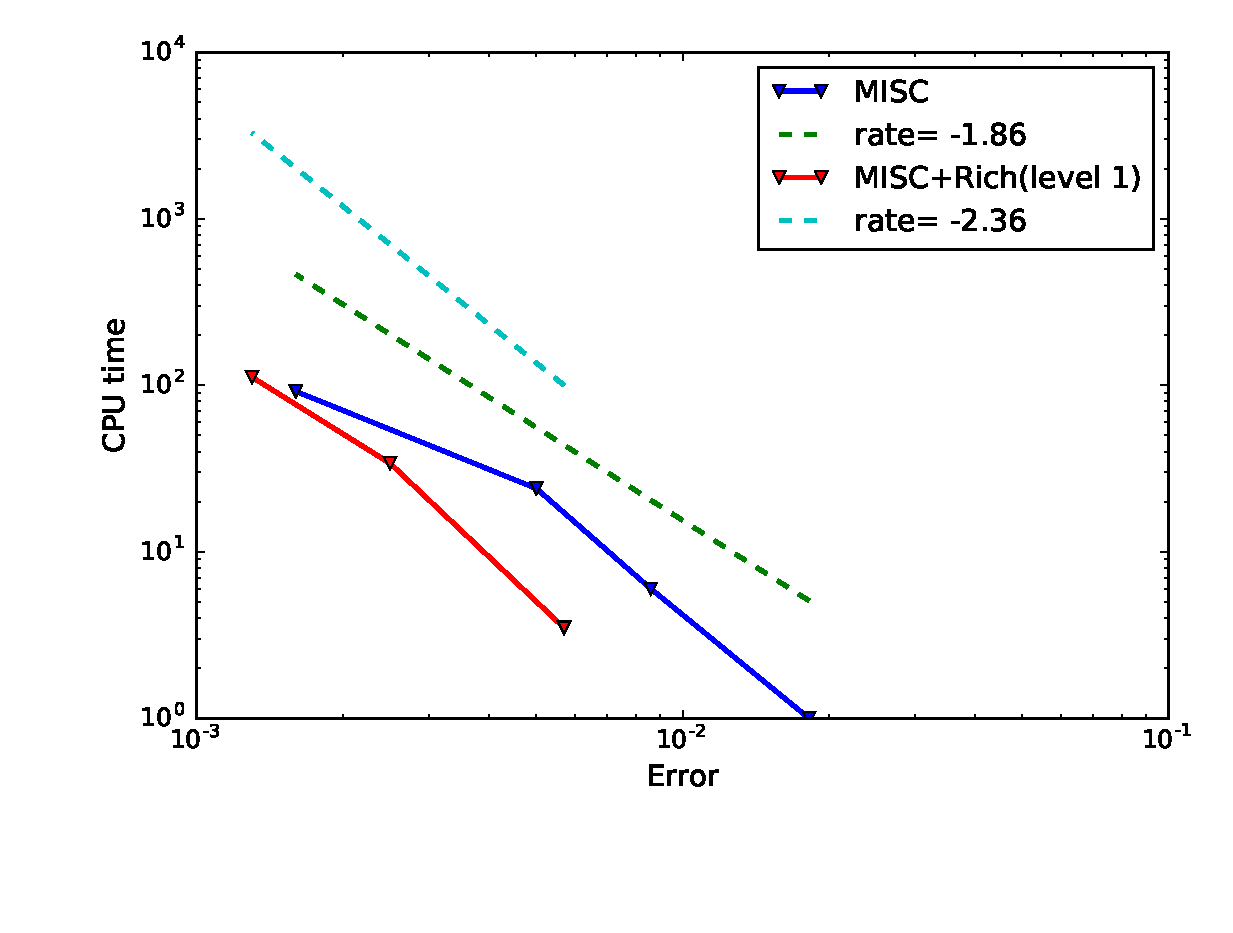
\includegraphics[width=0.5\linewidth]{./figures/rBergomi_Complexity_rates/set5/error_vs_time_set5_comparison}
	
	\caption{Complexity plot for  MISC (with/without) Richardson extrapolation for case set $3$ parameters of table \ref{table:Reference solution, using MC with $500$ time steps, of Call option price under rBergomi model, for different parameter constellation.}.}
	\label{fig:Complexity plot for  MISC for case set $3$ parameters, comparison}
\end{figure}







\FloatBarrier
\subsubsection{Case of set $4$ parameters in table \ref{table:Reference solution, using MC with $500$ time steps, of Call option price under rBergomi model, for different parameter constellation.}}\label{sec:Case of set 4 parameters}

\begin{table}[h!]
	\centering
	\begin{tabular}{l*{6}{c}r}
		Method \textbackslash  Steps            & $2$ & $4$ & $8$ & $16$ &   \\
		\hline
%		MISC ($TOL_{\text{MISC}}=5.10^{-1}$)  & $0.2413$ & $0.2403$ & $0.2403$ & $0.2396$  \\
		MISC ($TOL_{\text{MISC}}=10^{-1}$)  & $0.2413$ &$0.2403$& $0.2403$ & $0.2397$   \\
%		MISC ($TOL_{\text{MISC}}=5.10^{-2}$)  &$0.2413$ & $0.2403$ & $0.2403$ & $0.2406$  \\
		MISC ($TOL_{\text{MISC}}=10^{-2}$)  &$0.2413$ & $0.2403$ & $0.2409$ & $0.2413$  \\
		
		MISC ($TOL_{\text{MISC}}=10^{-3}$)  & $0.2413$ & $0.2411$ & $0.2414$ & $0.2413$  \\
		MISC ($TOL_{\text{MISC}}=10^{-4}$)  &  $0.2421$ & $0.2416$ & $0.2414$ & $-$  \\
		
		MISC ($TOL_{\text{MISC}}=10^{-5}$)  & $0.2421$ &$0.2416$ &  $0.2414$ & $-$  \\
		\hline
		MC method ($M=5.10^{6}$)   & $0.2420$ & $0.2416$  & $0.2414$ & $0.2413$ \\		
		
		\hline
	\end{tabular}
	\caption{ Call option price of the different methods for different number of time steps. Case set $4$ parameters in table \ref{table:Reference solution, using MC with $500$ time steps, of Call option price under rBergomi model, for different parameter constellation.}, without Richardson extrapolation.}
	\label{table: Call option price of the different methods for different number of time steps. Case set 4}
\end{table}


\begin{table}[h!]
	\centering
	\begin{tabular}{l*{6}{c}r}
		Method \textbackslash  Steps            & $2$ & $4$ & $8$ & $16$  \\
		\hline
		MC Bias ($M=5.10^6$)   & 	$ \underset{(    0.0013)}{\mathbf{0.0054}}$  & $\underset{(0.0008)}{\mathbf{0.0035
		}}$  & $\underset{(0.0007)}{\mathbf{0.0029}}$ & $\underset{(0.0006)}{\mathbf{0.0024}}$\\ 
		
		MC Statistical error ($M=5.10^6$)  &  $\underset{(   8.3e-05)} {\mathbf{3.4e-04}}$  & $\underset{(8.1e-05)} {\mathbf{3.4e-04}}$  & $\underset{(8.0e-05)} {\mathbf{3.3e-04 }}$ & $\underset{(8.0e-05)} {\mathbf{3.3e-04}}$	\\
		
		\hline
	\end{tabular}
	\caption{Bias and statistical errors of MC   for computing call option price  for different number of time steps. Case set $4$, without Richardson extrapolation. The numbers between parentheses are the corresponding absolute errors.}
	\label{Bias and Statistical errors of MC ($M=5.10^6$)  for computing Call option price  for different number of time steps. Case set 4, without Richardson extrapolation. The numbers between parentheses are the corresponding absolute errors.}
\end{table}





\begin{figure}[h!]
	\centering
	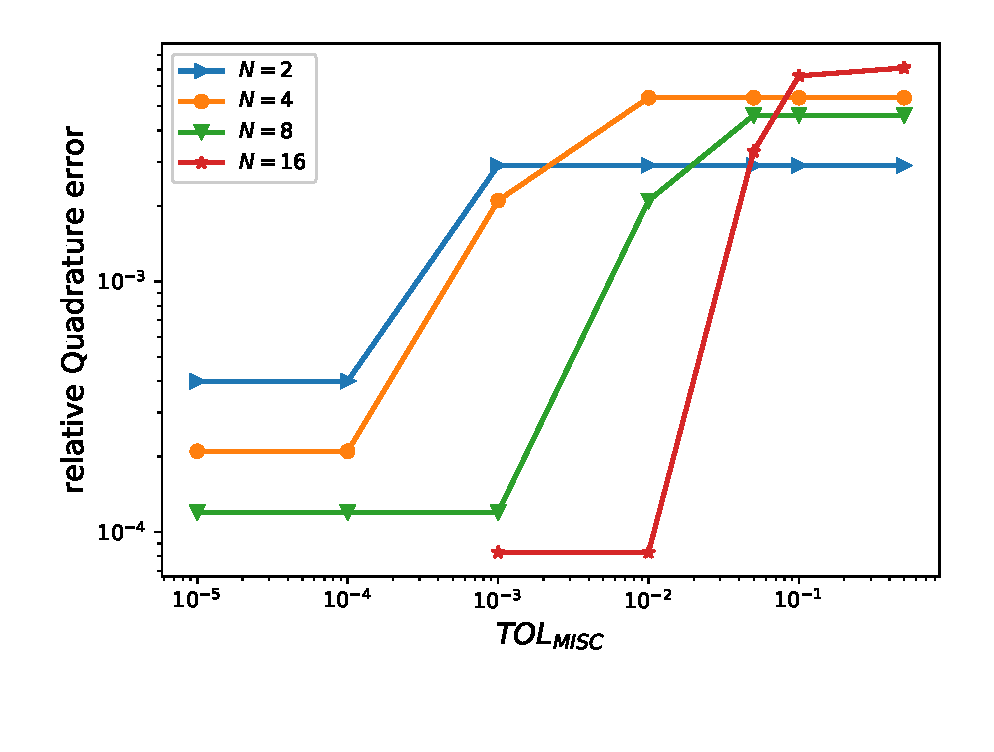
\includegraphics[width=0.5\linewidth]{./figures/rBergomi_MISC_quadratre_error/vs_TOL/set6/relative_quad_error_wrt_MISC_TOL_set6_non_rich}
	
	
	\caption{Quadrature error of MISC, with different tolerances, to compute call option price  for different number of time steps. Case  set $4$ parameters, without Richardson extrapolation.  See detailed values  in table \ref{Quadrature error of MISC to compute Call option price of the different tolerances for different number of time steps. Case  set $4$ parameters, without Richardson extrapolation. The numbers between parentheses are the corresponding absolute errors.}}
	\label{fig:Quadrature_error_set4}
\end{figure}





\begin{table}[h!]
	\centering
	\begin{tabular}{l*{6}{c}r}
		Method \textbackslash  Steps            & $2$ & $4$ & $8$ & $16$  \\
		\hline
%		MISC ($TOL_{\text{MISC}}=5.10^{-1}$)  & $\mathbf{0.0083}$ & $\mathbf{0.0089}$ & $\mathbf{ 0.0075}$ & $\mathbf{ 0.0095}$  \\
		MISC ($TOL_{\text{MISC}}=10^{-1}$)  &  $\mathbf{0.0083}$ & $\mathbf{0.0089}$& $\mathbf{ 0.0075}$ & $\mathbf{ 0.0090}$   \\
%		MISC ($TOL_{\text{MISC}}=5.10^{-2}$)  & $\mathbf{0.0083}$ & $\mathbf{0.0089}$ & $\mathbf{ 0.0075}$ & $\mathbf{ 0.0057}$  \\
		MISC ($TOL_{\text{MISC}}=10^{-2}$)  &  $\mathbf{0.0083}$ & $\mathbf{0.0089}$& $\mathbf{ 0.0050}$ & $\mathbf{ \red{0.0025}}$  \\
		MISC ($TOL_{\text{MISC}}=10^{-3}$)  &  $\mathbf{0.0083}$& $\mathbf{0.0056}$& $\mathbf{\red{0.0030}}$  & $\mathbf{ 0.0025}$  \\
		MISC ($TOL_{\text{MISC}}=10^{-4}$)  &  $\mathbf{\red{0.0058}}$ & $\mathbf{\red{0.0037}}$& $\mathbf{0.0030}$ & $\mathbf{ -}$ \\
		MISC ($TOL_{\text{MISC}}=10^{-5}$)  &  $\mathbf{0.0058}$ & $\mathbf{0.0037}$& $\mathbf{0.0030}$ & $\mathbf{ -}$ 
		\\
		\hline
		MC    & $\mathbf{\red{0.0057}}$  & $\mathbf{ \red{0.0038}}$  & $\mathbf{\red{0.0032}}$ & $\mathbf{ \red{0.0027}}$  \\		
		\hline
	\end{tabular}
	\caption{Total relative error of MISC,different tolerances, and MC to compute call option price  for different number of time steps. Case set $4$ parametrs of table \ref{table:Reference solution, using MC with $500$ time steps, of Call option price under rBergomi model, for different parameter constellation.}, without Richardson extrapolation. The numbers between parentheses are the corresponding absolute errors. The values marked in red, for MISC method, correspond to the total relative errors associated with  stable quadrature errors for MISC, and will be used for complexity comparison against MC.}
	\label{Total error of MISC and MC to compute Call option price of the different tolerances for different number of time steps. Case set 4, without Richardson extrapolation. The numbers between parentheses are the corresponding absolute errors.}
\end{table}


\begin{table}[h!]
	\centering
	\begin{tabular}{l*{6}{c}r}
		Method \textbackslash  Steps            & $2$ & $4$ & $8$ & $16$ &   \\
		\hline
%		MISC ($TOL_{\text{MISC}}=5.10^{-1}$)  & $0.1$ & $0.1$ & $0.1$ & $0.3$  \\
		MISC ($TOL_{\text{MISC}}=10^{-1}$)  & $0.1$ & $0.1$ & $0.1$ & $1$ \\
%		MISC ($TOL_{\text{MISC}}=5.10^{-2}$)  & $0.1$ & $0.1$ & $0.1$ & $22$  \\
		MISC ($TOL_{\text{MISC}}=10^{-2}$)  & $0.1$ & $0.15$ & $9$ & $\red{112}$ \\
		MISC ($TOL_{\text{MISC}}=10^{-3}$)  & $0.2$ & $2$ & $\red{27}$ & $2226$ \\
		MISC ($TOL_{\text{MISC}}=10^{-4}$)  & $\red{1}$ & $\red{6}$ & $136$ & $-$\\
		MISC ($TOL_{\text{MISC}}=10^{-5}$)  & $2$ & $18$ & $1559$ & $-$
		\\
		\hline
		MC method   & $ \red{141}
		
		$  & $  \red{246}$  & $  \red{461}$ & $ \red{820}
		$  \\	
		\hline
		Ratio of $\left(MC/MISC \right)$ & $ \red{141}
		
		$  & $  \red{
			41
		}$  & $  \red{    17
		}$ & $ \red{ 7}
		$  \\	
%		
		\hline
	\end{tabular}
	\caption{Comparison of the computational time (in Seconds) of  MC and MISC, used to compute call option price of rBergomi model for different number of time steps. Case set $4$ parameters of table \ref{table:Reference solution, using MC with $500$ time steps, of Call option price under rBergomi model, for different parameter constellation.}. The average  MC CPU time is computed over $10$ runs. }
	\label{Comparsion of the computational time of  MC and MISC, used to compute Call option price of rBergomi model for different number of time steps. Case set4}
\end{table}




	\begin{figure}[h!]
	\centering
	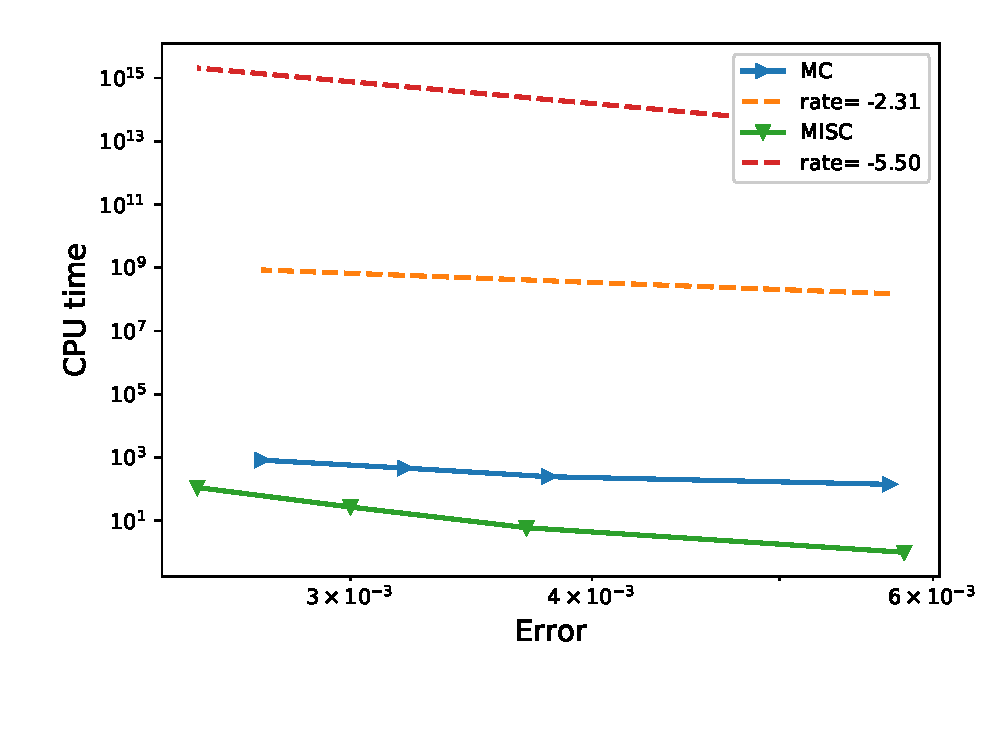
\includegraphics[width=0.5\linewidth]{./figures/rBergomi_Complexity_rates/set6/error_vs_time_set6}
	
	\caption{Complexity plot for   MC and MISC for case set $4$ parameters of table \ref{table:Reference solution, using MC with $500$ time steps, of Call option price under rBergomi model, for different parameter constellation.}.}
	\label{fig:Complexity plot for MC and MISC for case set $4$ parameters}
\end{figure}
\FloatBarrier
\subsubsection{Case of set $5$ parameters in table \ref{table:Reference solution, using MC with $500$ time steps, of Call option price under rBergomi model, for different parameter constellation.}}\label{sec:Case of set 5 parameters}

\begin{table}[h!]
	\centering
	\begin{tabular}{l*{6}{c}r}
		Method \textbackslash  Steps            & $2$ & $4$ & $8$ & $16$ &   \\
		\hline
%		MISC ($TOL_{\text{MISC}}=5.10^{-1}$)  & $0.0590$ & $0.0564$ & $0.0552$ & $0.0546$  \\
		MISC ($TOL_{\text{MISC}}=10^{-1}$)  & $0.0590$ &$0.0564$& $0.0552$ & $0.0546$   \\
%		MISC ($TOL_{\text{MISC}}=5.10^{-2}$)  &$0.0590$ & $0.0564$ & $0.0552$ & $0.0557$  \\
		MISC ($TOL_{\text{MISC}}=10^{-2}$)  &$0.0590$ &$0.0564$ & $0.0574$ & $0.0572$  \\
		
		MISC ($TOL_{\text{MISC}}=10^{-3}$)  & $0.0605$ & $0.0587$ & $0.0579$ & $0.0575$  \\
		MISC ($TOL_{\text{MISC}}=10^{-4}$)  &  $0.0605$ & $0.0587$ & $0.0576$ & $-$  \\
		
		MISC ($TOL_{\text{MISC}}=10^{-5}$)  & $0.0605$ & $0.0587$ &  $0.0579$ & $-$  \\
		\hline
		MC method ($M=5.10^{6}$)   & $0.0605$ & $0.0587$  & $0.0579$ & $0.0576$ \\		
		
		\hline
	\end{tabular}
	\caption{ Call option price of the different methods for different number of time steps. Case of set $5$ parameters in table \ref{table:Reference solution, using MC with $500$ time steps, of Call option price under rBergomi model, for different parameter constellation.}, without Richardson extrapolation.}
	\label{table: Call option price of the different methods for different number of time steps. Case set 5}
\end{table}


\begin{table}[h!]
	\centering
	\begin{tabular}{l*{6}{c}r}
		Method \textbackslash  Steps            & $2$ & $4$ & $8$ & $16$  \\
		\hline
		MC Bias ($M=5.10^6$)   & 	$ \underset{(0.0037
			)}{\mathbf{0.0650}}$  & $\underset{(0.0019)}{\mathbf{0.0330
		}}$  & $\underset{(0.0012)}{\mathbf{0.0202}}$ & $\underset{(0.0007)}{\mathbf{0.0130}}$\\ 
		
		MC Statistical error ($M=5.10^6$)  &  $\underset{(   4.0e-05)} {\mathbf{7.0e-04}}$  & $\underset{(3.8e-05)} {\mathbf{6.7e-04}}$  & $\underset{(3.7e-05)} {\mathbf{6.5e-04 }}$ & $\underset{(3.6e-05)} {\mathbf{6.3e-04}}$	\\
		
		\hline
	\end{tabular}
	\caption{Bias and statistical errors of MC   for computing call option price  for different number of time steps. Case set $5$, without Richardson extrapolation. The numbers between parentheses are the corresponding absolute errors.}
	\label{Bias and Statistical errors of MC ($M=5.10^6$)  for computing Call option price  for different number of time steps. Case set 5, without Richardson extrapolation. The numbers between parentheses are the corresponding absolute errors.}
\end{table}
%
%
%








\begin{figure}[h!]
	\centering
	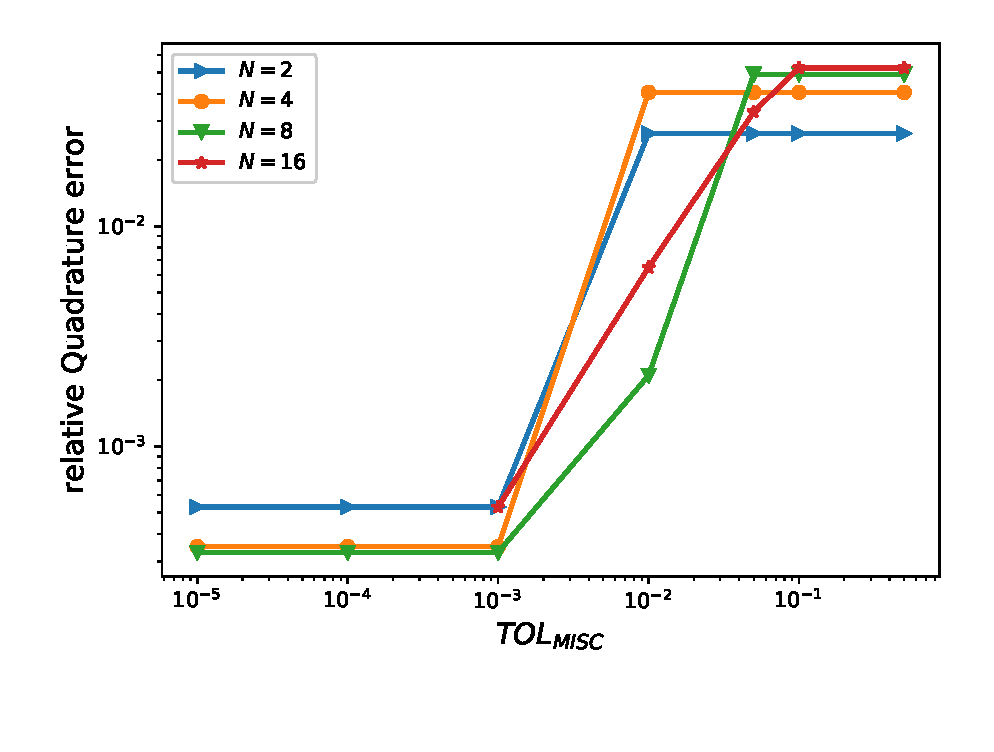
\includegraphics[width=0.5\linewidth]{./figures/rBergomi_MISC_quadratre_error/vs_TOL/set7/relative_quad_error_wrt_MISC_TOL_set7_non_rich}
	
	
	\caption{Quadrature error of MISC, with  different tolerances,  to compute call option price  for different number of time steps. Case  set $5$ parameters, without Richardson extrapolation.  See detailed values  in table \ref{Quadrature error of MISC to compute Call option price of the different tolerances for different number of time steps. Case  set $5$ parameters, without Richardson extrapolation. The numbers between parentheses are the corresponding absolute errors.}}
	\label{fig:Quadrature_error_set5}
\end{figure}


%
%
%
\begin{table}[h!]
	\centering
	\begin{tabular}{l*{6}{c}r}
		Method \textbackslash  Steps            & $2$ & $4$ & $8$ & $16$  \\
		\hline
%		MISC ($TOL_{\text{MISC}}=5.10^{-1}$)  & $\mathbf{0.0914}$ & $\mathbf{0.0736}$ & $\mathbf{ 0.0693}$ & $\mathbf{ 0.0654}$  \\
		MISC ($TOL_{\text{MISC}}=10^{-1}$)  & $\mathbf{0.0914}$ & $\mathbf{0.0736}$& $\mathbf{ 0.0693}$ & $\mathbf{ 0.0654}$   \\
%		MISC ($TOL_{\text{MISC}}=5.10^{-2}$)  & $\mathbf{0.0914}$ & $\mathbf{0.0736}$ & $\mathbf{ 0.0693}$ & $\mathbf{ 0.0461}$  \\
		MISC ($TOL_{\text{MISC}}=10^{-2}$)  &  $\mathbf{0.0914}$& $\mathbf{0.0736}$& $\mathbf{ 0.0223}$ & $\mathbf{ 0.0195}$  \\
		MISC ($TOL_{\text{MISC}}=10^{-3}$)  &  $\mathbf{\red{0.0655}}$& $\mathbf{\red{0.0334}}$& $\mathbf{\red{0.0205}}$  & $\mathbf{ \red{0.0135}}$  \\
		MISC ($TOL_{\text{MISC}}=10^{-4}$)  &  $\mathbf{0.0655}$& $\mathbf{0.0334}$& $\mathbf{0.0205}$ & $\mathbf{ -}$ \\
		MISC ($TOL_{\text{MISC}}=10^{-5}$)  &  $\mathbf{0.0655}$ & $\mathbf{0.0334}$& $\mathbf{0.0205}$ & $\mathbf{ -}$ 
		\\
		\hline
		MC    & $\mathbf{\red{0.0657}}$  & $\mathbf{ \red{0.0337}}$  & $\mathbf{\red{0.0209}}$ & $\mathbf{ \red{0.0136}}$  \\		
		\hline
	\end{tabular}
	\caption{Total relative error of MISC, with  different tolerances,  and MC to compute call option price  for different number of time steps. Case  set $5$ parametrs of table \ref{table:Reference solution, using MC with $500$ time steps, of Call option price under rBergomi model, for different parameter constellation.}, without Richardson extrapolation. The numbers between parentheses are the corresponding absolute errors. The values marked in red, for MISC method, correspond to the total relative errors associated with  stable quadrature errors for MISC, and will be used for complexity comparison against MC.}
	\label{Total error of MISC and MC to compute Call option price of the different tolerances for different number of time steps. Case set 5, without Richardson extrapolation. The numbers between parentheses are the corresponding absolute errors.}
\end{table}


\begin{table}[h!]
	\centering
	\begin{tabular}{l*{6}{c}r}
		Method \textbackslash  Steps            & $2$ & $4$ & $8$ & $16$ &   \\
		\hline
%		MISC ($TOL_{\text{MISC}}=5.10^{-1}$)  & $0.1$ & $0.1$ & $0.2$ & $0.5$  \\
		MISC ($TOL_{\text{MISC}}=10^{-1}$)  & $0.1$ & $0.1$ & $0.2$ & $0.5$ \\
%		MISC ($TOL_{\text{MISC}}=5.10^{-2}$)  & $0.1$ & $0.1$ & $0.2$ & $5$  \\
		MISC ($TOL_{\text{MISC}}=10^{-2}$)  & $0.1$ & $0.1$ & $8$ & $97$ \\
		MISC ($TOL_{\text{MISC}}=10^{-3}$)  & $\red{0.7}$ & $\red{4}$ & $\red{26}$ & $\red{1984}$ \\
		MISC ($TOL_{\text{MISC}}=10^{-4}$)  & $1$ & $8$ & $173$ & $-$\\
		MISC ($TOL_{\text{MISC}}=10^{-5}$)  & $1$ & $32$ & $2129$ & $-$
		\\
		\hline
		MC method   & $ \red{154}
		
		$  & $  \red{229}$  & $  \red{420}$ & $ \red{938}
		$  \\	
		\hline
		Ratio of $\left(MC/MISC \right)$ & $ \red{   220}
		
		$  & $  \red{
		 57
		}$  & $  \red{    16
		}$ & $ \red{ 0.5}
		$  \\	
				
		\hline
	\end{tabular}
	\caption{Comparison of the computational time (In seconds) of  MC and MISC, used to compute Call option price of rBergomi model for different number of time steps. Case set $5$ parametrs of table \ref{table:Reference solution, using MC with $500$ time steps, of Call option price under rBergomi model, for different parameter constellation.}. The average  MC CPU time is computed over $10$ runs. }
	\label{Comparsion of the computational time of  MC and MISC, used to compute Call option price of rBergomi model for different number of time steps. Case set5}
\end{table}
	\begin{figure}[h!]
	\centering
	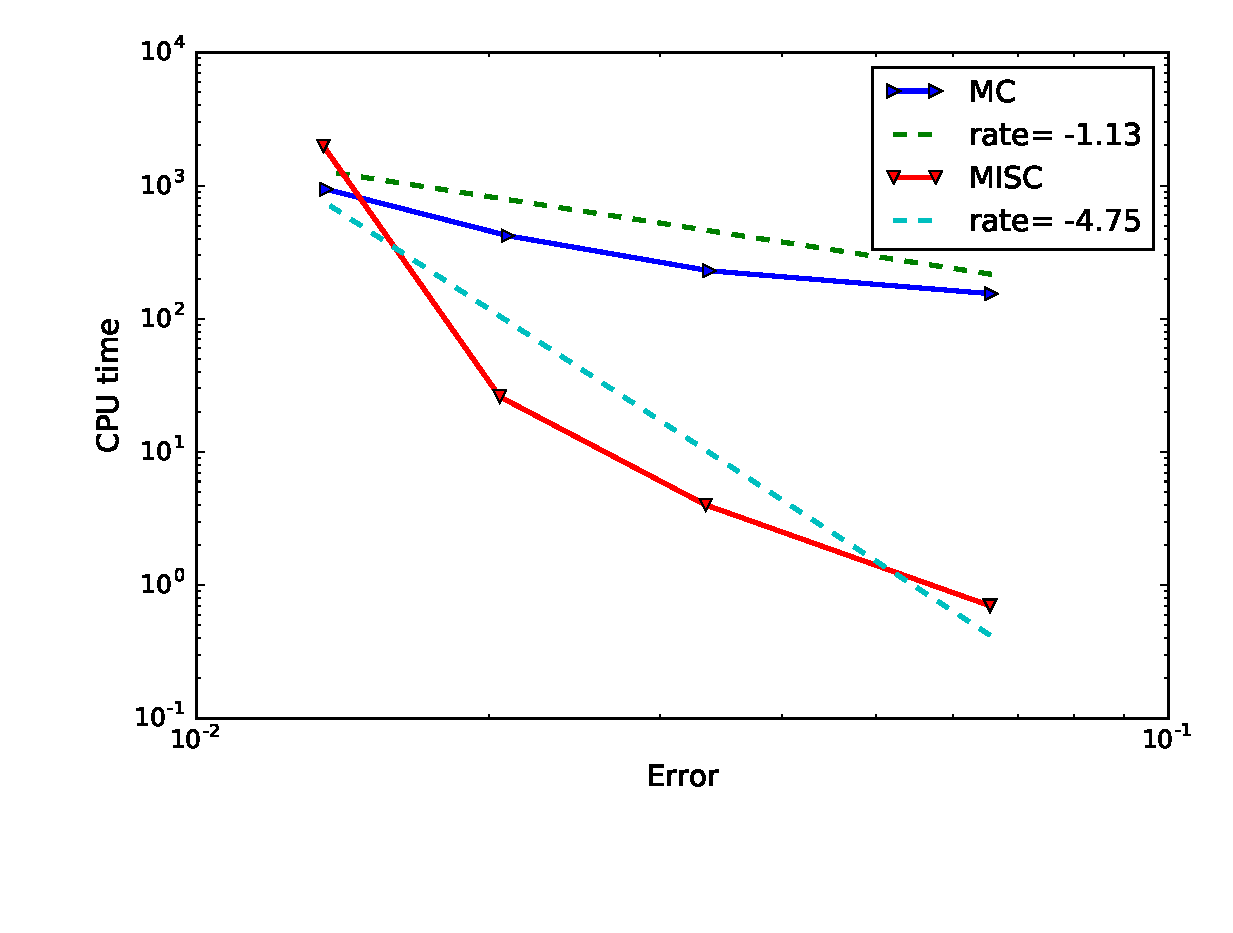
\includegraphics[width=0.5\linewidth]{./figures/rBergomi_Complexity_rates/set7/error_vs_time_set7}
	
	\caption{Complexity plot for   MC and MISC for case set $5$ parameters of table \ref{table:Reference solution, using MC with $500$ time steps, of Call option price under rBergomi model, for different parameter constellation.}.}
	\label{fig:Complexity plot for MC and MISC for Case set $5$ parameters}
\end{figure}
\FloatBarrier



